% This must be in the first 5 lines to tell arXiv to use pdfLaTeX, which is strongly recommended.
% \pdfoutput=1  % Commented out for XeLaTeX compilation
% In particular, the hyperref package requires pdfLaTeX in order to break URLs across lines.

\documentclass[11pt]{article}

% Change "review" to "final" to generate the final (sometimes called camera-ready) version.
% Change to "preprint" to generate a non-anonymous version with page numbers.
\usepackage[preprint]{acl}

% Standard package includes
\usepackage{times}
\usepackage{latexsym}
\usepackage{amsmath}
\usepackage{amssymb}
\usepackage{xcolor}
\usepackage{booktabs}
% For proper rendering and hyphenation of words containing Latin characters (including in bib files)
% \usepackage[T1]{fontenc}  % Not needed for XeLaTeX
% For Vietnamese characters
% \usepackage[T5]{fontenc}
% See https://www.latex-project.org/help/documentation/encguide.pdf for other character sets

% This assumes your files are encoded as UTF8
% \usepackage[utf8]{inputenc}  % Not needed for XeLaTeX

% For Chinese character support in XeLaTeX
\usepackage{xeCJK}
% 设置中文字体,按优先级尝试不同字体
\setCJKmainfont[
    BoldFont={SimHei},
    ItalicFont={KaiTi}
]{SimSun}

% 将摘要标题从 "Abstract" 改为 "摘要"
\renewcommand{\abstractname}{摘要}

% This is not strictly necessary, and may be commented out,
% but it will improve the layout of the manuscript,
% and will typically save some space.
\usepackage{microtype}
\usepackage{tcolorbox}
% This is also not strictly necessary, and may be commented out.
% However, it will improve the aesthetics of text in
% the typewriter font.
\usepackage{inconsolata}

%Including images in your LaTeX document requires adding
%additional package(s)
\usepackage{graphicx}

\def\retrievaltextcircled#1{\large{\textcircled{\small{\color{blue}#1}}}\normalsize}
\def\reranktextcircled#1{\large{\textcircled{\small{\textcolor{red}{#1}}}}\normalsize}
\def\datatextcircled#1{\large{\textcircled{\small{#1}}}\normalsize}
\def\fusiontextcircled#1{\large{\textcircled{\small{\color{green}#1}}}\normalsize}
\def\mergetextcircled#1{\large{\textcircled{\small{\color{orange}#1}}}\normalsize}
\def\doctextcircled#1{\large{\textcircled{\small{\color{purple}#1}}}\normalsize}

% If the title and author information does not fit in the area allocated, uncomment the following
%
%\setlength\titlebox{<dim>}
%
% and set <dim> to something 5cm or larger.

\title{MicroRCA-Agent: 基于大模型智能体的微服务根因定位方法}

% Author information can be set in various styles:
% For several authors from the same institution:
% \author{Author 1 \and ... \and Author n \\
%         Address line \\ ... \\ Address line}
% if the names do not fit well on one line use
%         Author 1 \\ {\bf Author 2} \\ ... \\ {\bf Author n} \\
% For authors from different institutions:
% \author{Author 1 \\ Address line \\  ... \\ Address line
%         \And  ... \And
%         Author n \\ Address line \\ ... \\ Address line}
% To start a separate ``row'' of authors use \AND, as in
% \author{Author 1 \\ Address line \\  ... \\ Address line
%         \AND
%         Author 2 \\ Address line \\ ... \\ Address line \And
%         Author 3 \\ Address line \\ ... \\ Address line}
\author{
    %Authors
    % All authors must be in the same font size and format.
    Pan Tang\textsuperscript{\rm 1}\thanks{\ \ Corresponding author}, Shixiang Tang\textsuperscript{\rm 1}, Huanqi Pu\textsuperscript{\rm 1},\bf {Zhiqing Miao\textsuperscript{\rm 1}, Zhixing Wang\textsuperscript{\rm 1}}\\
    \textsuperscript{\rm 1}CCSE, School of Computer Science and Engineering, Beihang University, Beijing, China\\
    % \textsuperscript{\rm 2}Zhongguancun Laboratory, Beijing, China\\
    \texttt{\{zcmuller,kuangdd,wangzy23,hiyouga\}@buaa.edu.cn}, \texttt{\{niezj,zhangrc\}@act.buaa.edu.cn}
}

%\author{
%  \textbf{First Author\textsuperscript{1}},
%  \textbf{Second Author\textsuperscript{1,2}},
%  \textbf{Third T. Author\textsuperscript{1}},
%  \textbf{Fourth Author\textsuperscript{1}},
%\\
%  \textbf{Fifth Author\textsuperscript{1,2}},
%  \textbf{Sixth Author\textsuperscript{1}},
%  \textbf{Seventh Author\textsuperscript{1}},
%  \textbf{Eighth Author \textsuperscript{1,2,3,4}},
%\\
%  \textbf{Ninth Author\textsuperscript{1}},
%  \textbf{Tenth Author\textsuperscript{1}},
%  \textbf{Eleventh E. Author\textsuperscript{1,2,3,4,5}},
%  \textbf{Twelfth Author\textsuperscript{1}},
%\\
%  \textbf{Thirteenth Author\textsuperscript{3}},
%  \textbf{Fourteenth F. Author\textsuperscript{2,4}},
%  \textbf{Fifteenth Author\textsuperscript{1}},
%  \textbf{Sixteenth Author\textsuperscript{1}},
%\\
%  \textbf{Seventeenth S. Author\textsuperscript{4,5}},
%  \textbf{Eighteenth Author\textsuperscript{3,4}},
%  \textbf{Nineteenth N. Author\textsuperscript{2,5}},
%  \textbf{Twentieth Author\textsuperscript{1}}
%\\
%\\
%  \textsuperscript{1}Affiliation 1,
%  \textsuperscript{2}Affiliation 2,
%  \textsuperscript{3}Affiliation 3,
%  \textsuperscript{4}Affiliation 4,
%  \textsuperscript{5}Affiliation 5
%\\
%  \small{
%    \textbf{Correspondence:} \href{mailto:email@domain}{email@domain}
%  }
%}

% 设置四级标题paragraph的编号和格式
\setcounter{secnumdepth}{4} % 设置编号深度到paragraph级别
\setcounter{tocdepth}{4}    % 设置目录深度到paragraph级别

% 定义paragraph的编号格式
\renewcommand{\theparagraph}{\thesubsubsection.\arabic{paragraph}}

% 设置paragraph标题的格式
\makeatletter
\renewcommand{\paragraph}{%
    \@startsection{paragraph}{4}{\z@}%
    {3.25ex \@plus1ex \@minus.2ex}%
    {1.5ex \@plus.2ex}%
    {\normalfont\normalsize\bfseries}%
}
\makeatother

\begin{document}
\maketitle
\begin{abstract}
本文提出了MicroRCA-Agent,一套基于大模型智能体的微服务根因定位创新解决方案,构建了多模态数据融合的智能故障根因定位系统。技术创新主要体现在三个方面:首先,结合预训练Drain日志解析算法与多重筛选机制,将海量日志高效压缩为高质量故障特征;其次,采用IsolationForest无监督学习算法和状态码检查相结合的方式,实现调用链的双重异常识别;最后,设计统计对称比率过滤机制和双层级LLM分析策略,实现node-service-pod三层次的全栈现象总结。多模态根因分析模块通过精心设计的跨模态提示词,深度融合多模态异常信息,充分利用大语言模型的跨模态理解和逻辑推理能力,输出包含故障组件、根因描述和推理过程的结构化分析结果。消融实验充分验证了各模态数据的互补价值和系统架构的有效性,该方案在复杂微服务故障场景中表现优异,最终获得50.71分的成绩。代码已开源至:\url{https://github.com/tangpan360/MicroRCA-Agent}。

\end{abstract}

\section{总体设计}
\label{sec:design}
本方案采用模块化架构设计,整体系统分为五个核心模块:数据预处理模块、日志故障抽取模块、追踪故障检测模块、指标故障总结模块和多模态根因分析模块。各模块间采用松耦合设计,通过函数封装进行数据交互,既保证了系统的整体性,又确保了各模块的独立性和可扩展性。

数据预处理模块承担着系统数据标准化的关键职责。核心功能包括:从input.json中解析故障时间段信息;对log、trace、metric三种模态的原始数据进行时间戳格式统一,确保后续跨模态数据关联的准确性。

Log故障抽取模块基于“模板化+规则化”的处理架构。首先构建分层次故障模板体系,设计了多条覆盖不同故障类型的正则表达式规则,包括完整错误消息与错误代码组合、错误类型与请求路径组合、异常类型区分等多个层级。利用预训练的 Drain 模型\cite{he2017drain}(error\_log-drain.pkl)进行日志模板自动提取,通过模板识别与去重机制,将相同语义的日志条目合并为模板及其出现次数的形式,并可通过 drain3.ini 配置文件精确控制模板匹配参数。该模块实现多重筛选机制:文件定位→时间窗过滤→error关键词过滤→核心字段提取与重构→故障模板匹配与标准化→样本去重与频次统计→名字映射与service提取,有效将海量原始日志压缩为高质量故障特征。

\begin{figure*}[t]
    \centering
    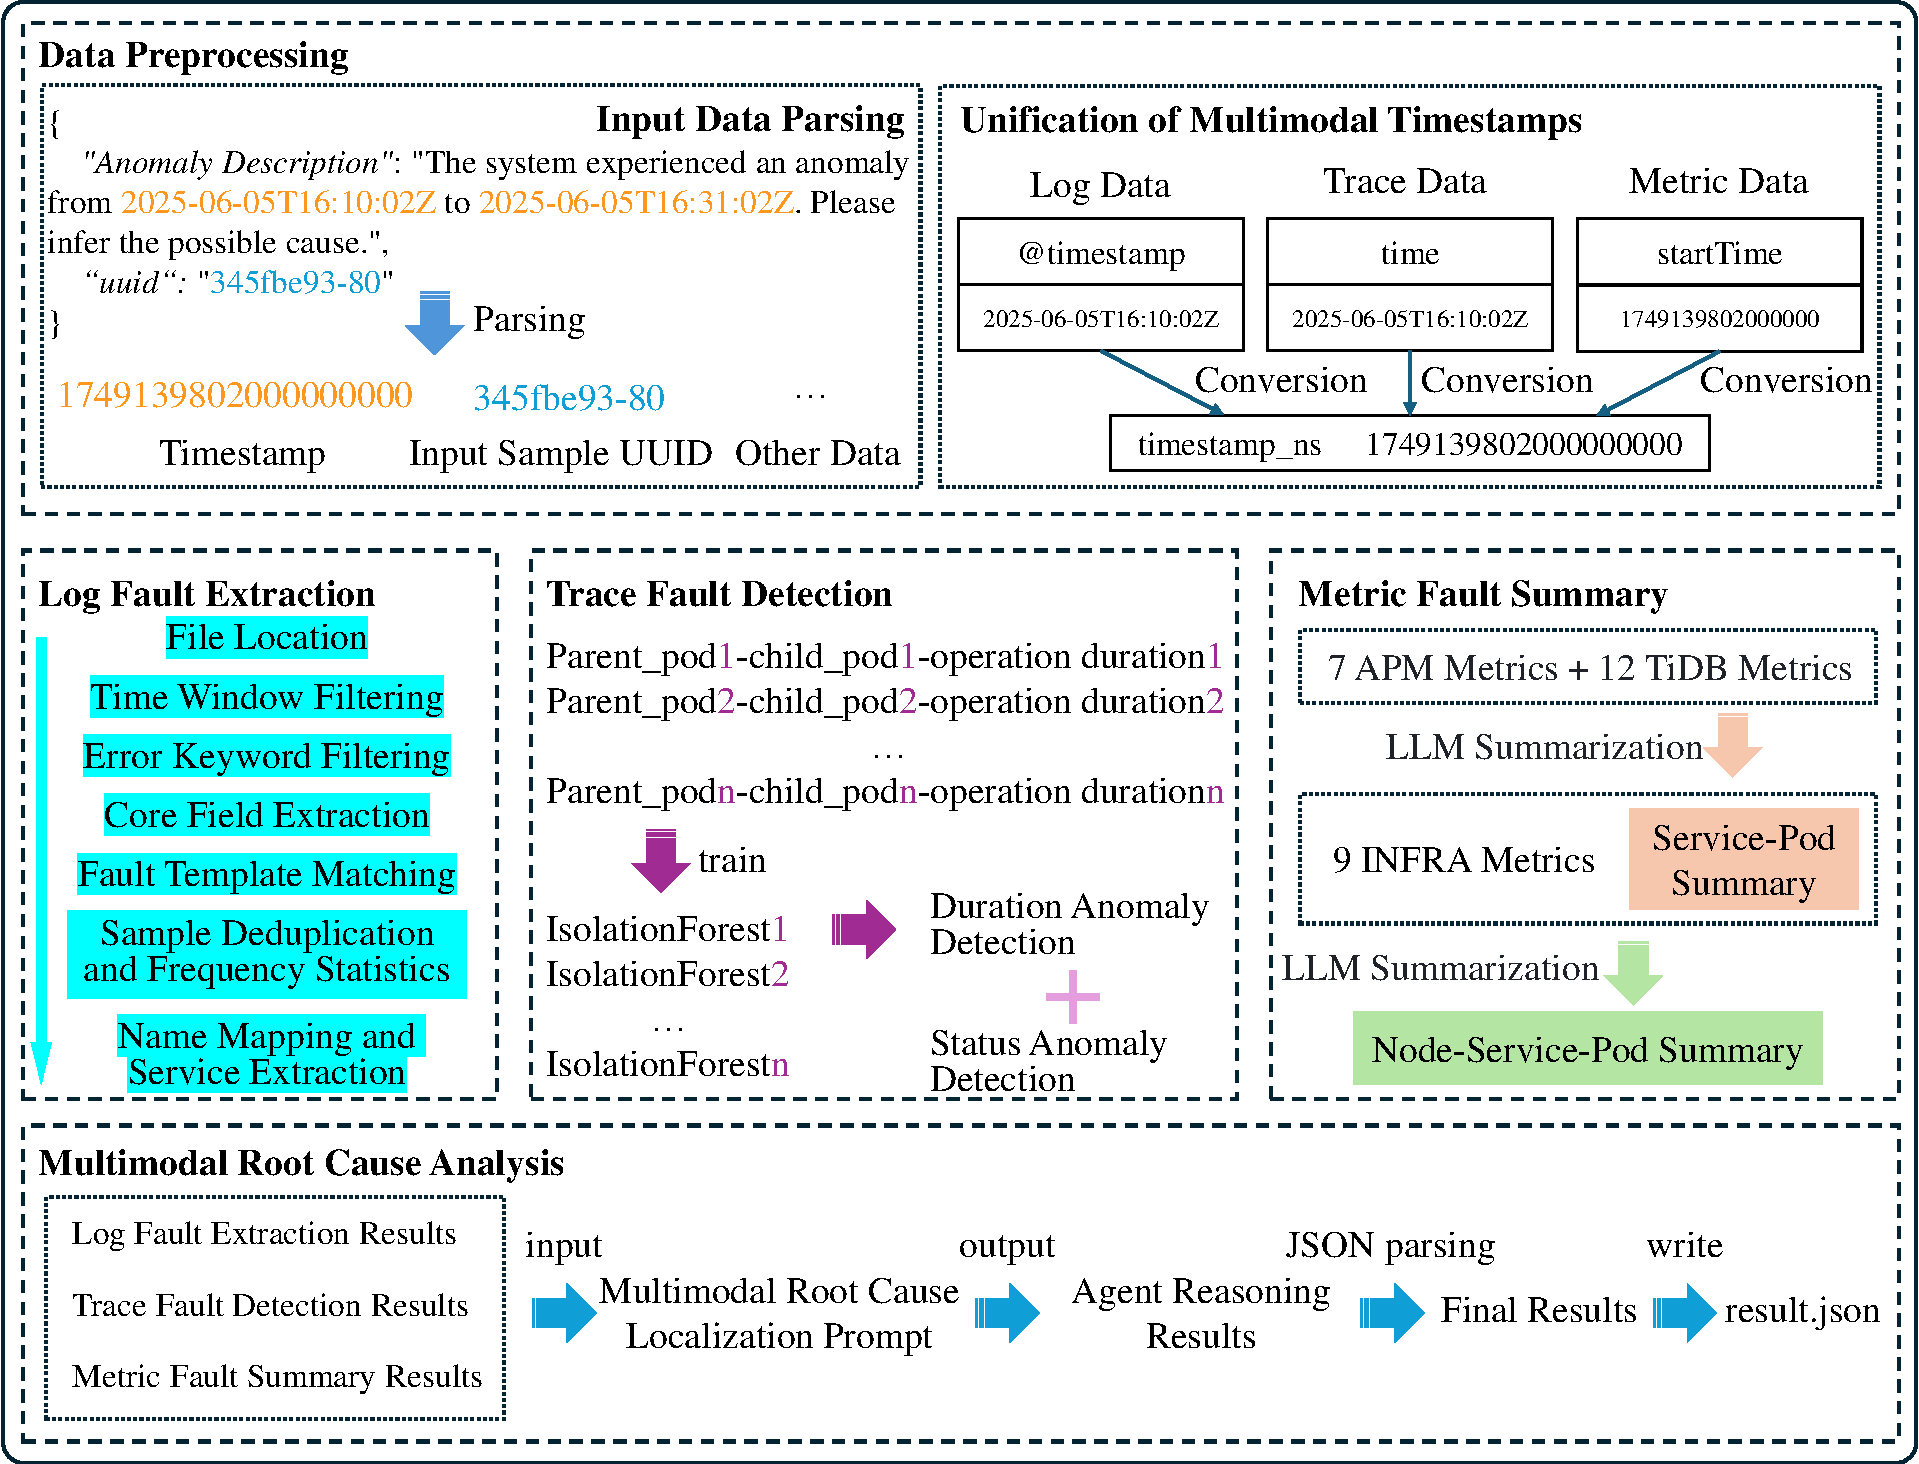
\includegraphics[width=0.95\linewidth]{pics/fig1.pdf}
    \caption{MicroRCA-Agent系统总体架构}
    \label{fig1}
\end{figure*}

\begin{figure*}[htbp]
    \centering
    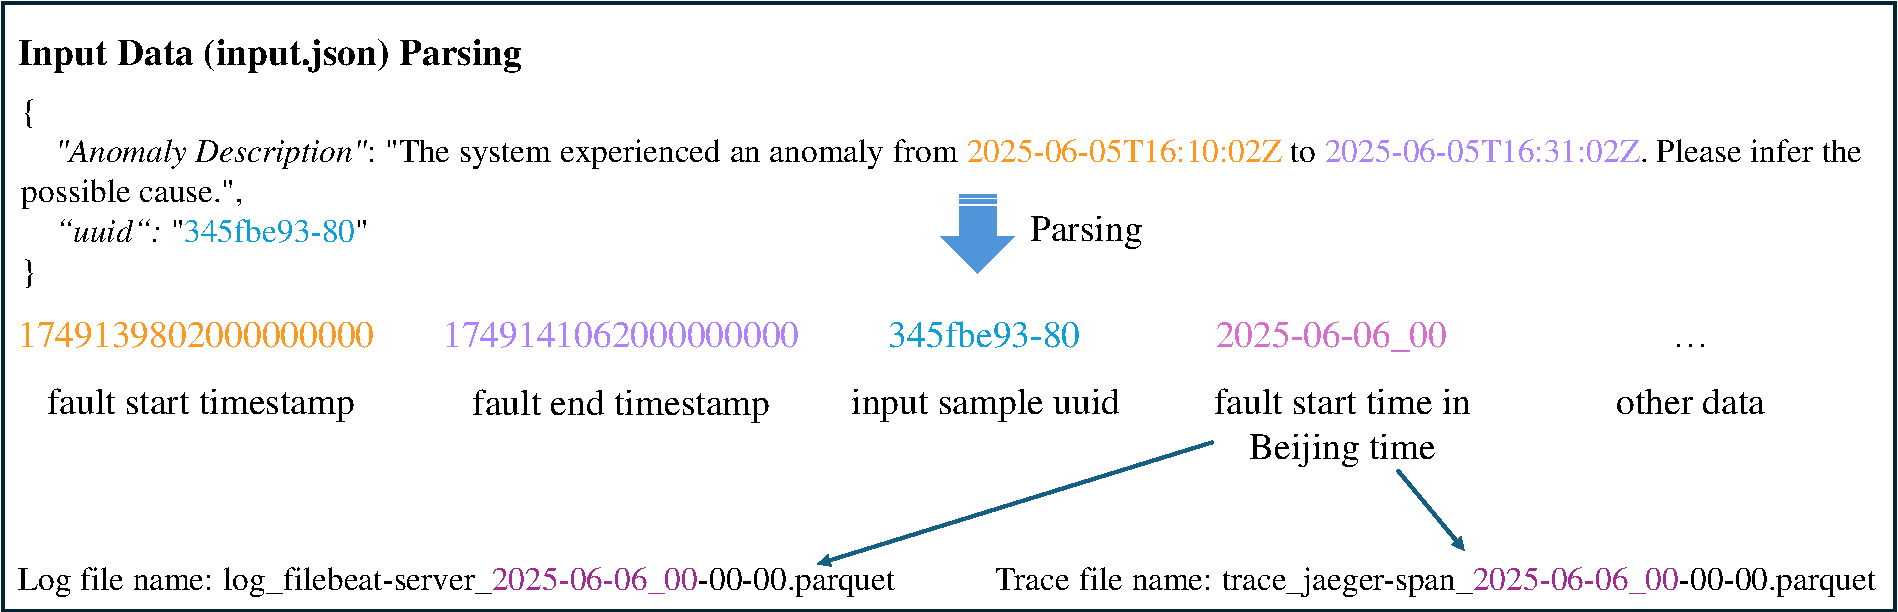
\includegraphics[width=0.95\linewidth]{pics/fig2.pdf}
    \caption{输入数据解析}
    \label{fig2}
\end{figure*}

Trace故障检测模块采用“无监督学习+规则增强”的混合检测策略。核心基于IsolationForest\cite{liu2008isolation}算法构建异常检测模型,利用正常时期parent\_pod→chile\_pod调用链的duration数据进行模型训练。使用50个随机样本提取正常数据,采用30秒滑动窗口提取时序特征,训练生成trace\_detectors.pkl模型文件。检测阶段对故障期间parent\_pod→chile\_pod调用链的duration进行异常检测,筛选出明显异常的调用链和其duration。同时实现status组合分析功能,提取trace中的status.code和status.message信息,识别调用失败模式。最终分别输出出现次数最多的前20个异常调用组合的统计分析和前20个详细的status异常信息。

Metric故障总结模块设计了统计对称比率过滤结合层次化两阶段的LLM分析策略。首先对于Metric指标进行数学统计分析,并借助对称比率判断正常区间和故障区间数据统计指标是否高度相似,以此过滤正常数据,大幅度降低大模型上下文长度,使其更关注可能的异常数据,过滤后进行两阶段LLM分析,第一阶段基于应用性能监控数据(APM)和数据库组件(TiDB)数据,分别进行了service级别和pod级别的现象总结,包括微服务的请求相应、异常比例等业务指标,以及数据库附属组件TiDB、TiKV和PD等相关指标。第二阶段将第一阶段的业务指标现象总结与Node级别的基础设施数据相结合,进行service,pod,node三层次的现象综合分析。在保证分析深度的同时有效控制计算成本。



\begin{figure*}[htbp]
    \centering
    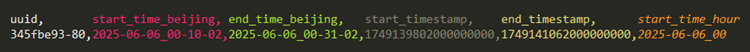
\includegraphics[width=0.95\textwidth]{pics/fig3.png}
    \caption{预处理后的input数据}
    \label{fig3}
\end{figure*}


多模态根因分析模块核心设计了专门的多模态提示词,支持log、trace和metric三种模态数据的灵活组合。该模块采用多进程策略提升系统处理效率,集成了完整的容错机制和重试策略。最终输出包含component、reason、reasoning\_trace的结构化根因分析结果,实现从现象观察到根因推理的完整闭环。


\section{创新性和实用性}
\label{sec:innovation}

本方案在创新性上体现在多层次特征提取与推理架构设计上。首先,日志、调用链与指标模块分别采用针对性较强的处理与筛选策略:Drain算法结合多级过滤来压缩日志冗余;IsolationForest与状态码检查互补识别trace异常;统计显著性筛选高价值metric特征。这种分模态“精准抽取—信息压缩”机制,在保证关键信息完整性的同时,显著降低了后续分析的计算与上下文开销。其次,指标分析部分设计了统计对称比率法过滤机制和双层级现象总结框架,在过滤出可能异常数据后,将服务/实例和容器/节点两类视角有机结合,并在现象层面保留业务与基础设施的关联脉络,为后续根因定位提供直接可用的语义化证据。

在实用性方面,本方案突出了模块化和可扩展性设计,能够灵活适配不同业务与系统环境。各功能模块(日志抽取、调用链检测、指标总结、根因分析)相互解耦,既可独立部署,也可按需组合,方便在不同规模与复杂度的微服务架构中快速落地。在处理效率上,方案通过分层筛选等策略,大幅减少无关数据进入分析环节,降低计算与存储开销,适合高并发、大数据量的生产环境。


\section{详细设计}
\label{sec:detail}

本方案围绕微服务系统的故障根因定位需求,构建了由数据预处理、log故障抽取、trace故障检测、metric故障总结和多模态根因分析五个模块组成的完整系统结构(如图\ref{fig1}所示)。系统首先通过数据预处理模块实现输入故障信息的结构化解析和多模态时间戳统一;随后log模块从大规模日志多层级筛选,并利用drain提取日志模板去重,trace模块采用duration性能与状态双策略识别调用异常,metric模块借助大模型实现多层级监控指标的现象总结;最终,所有模态数据汇聚至多模态根因分析模块,通过大语言模型的跨模态推理能力,实现对故障组件的定位、原因的解释与证据链条的输出。

\begin{figure*}[htbp]
    \centering
    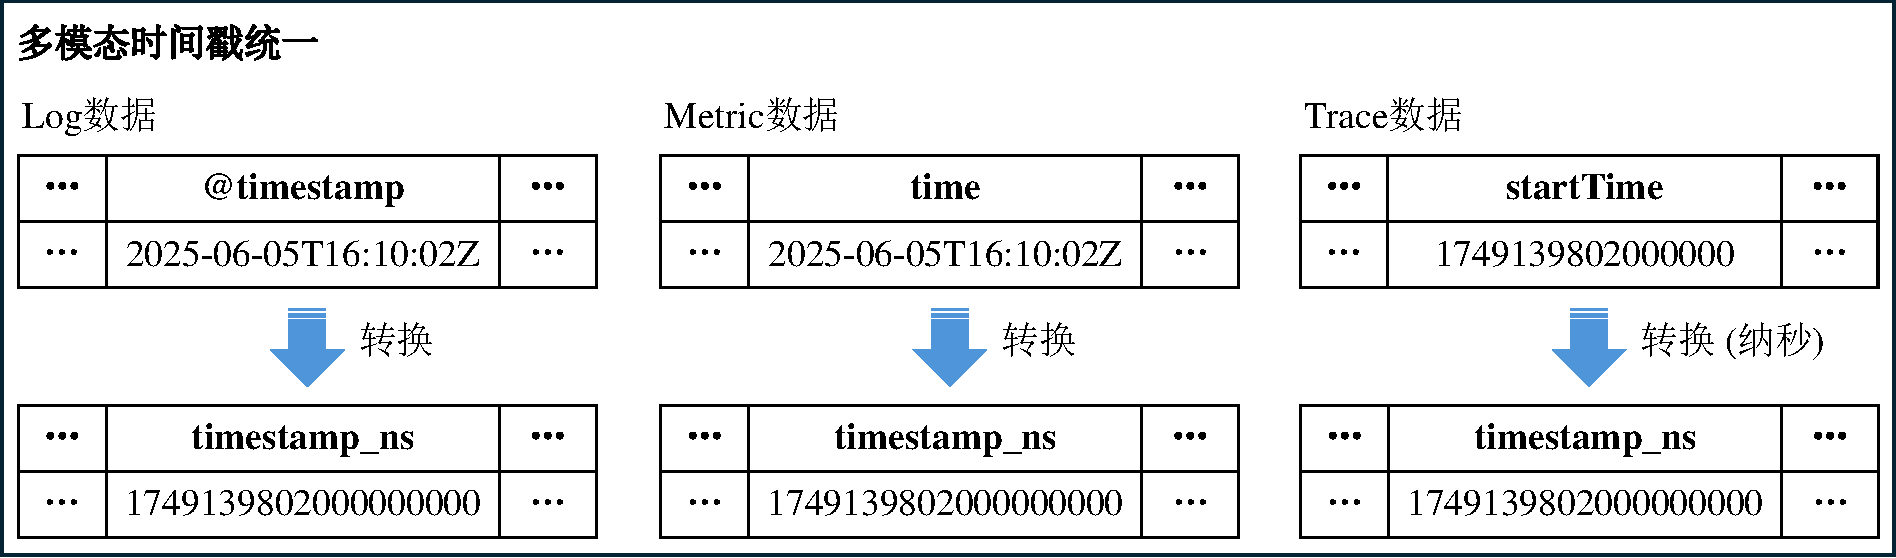
\includegraphics[width=0.95\textwidth]{pics/fig4.pdf}
    \caption{多模态数据时间戳统一}
    \label{fig4}
\end{figure*}

\begin{figure*}[htbp]
    \centering
    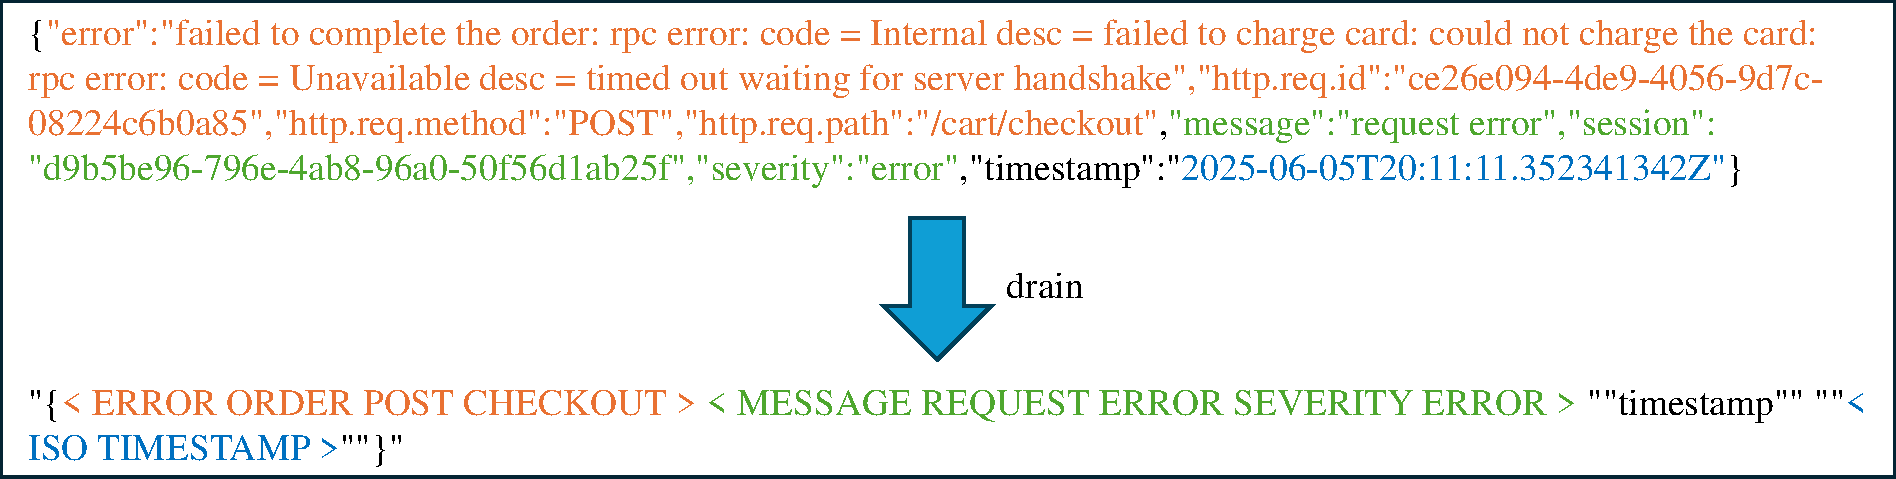
\includegraphics[width=0.95\textwidth]{pics/fig5.pdf}
    \caption{Drain 提取日志模板}
    \label{fig5}
\end{figure*}

\begin{figure*}[htbp]
    \centering
    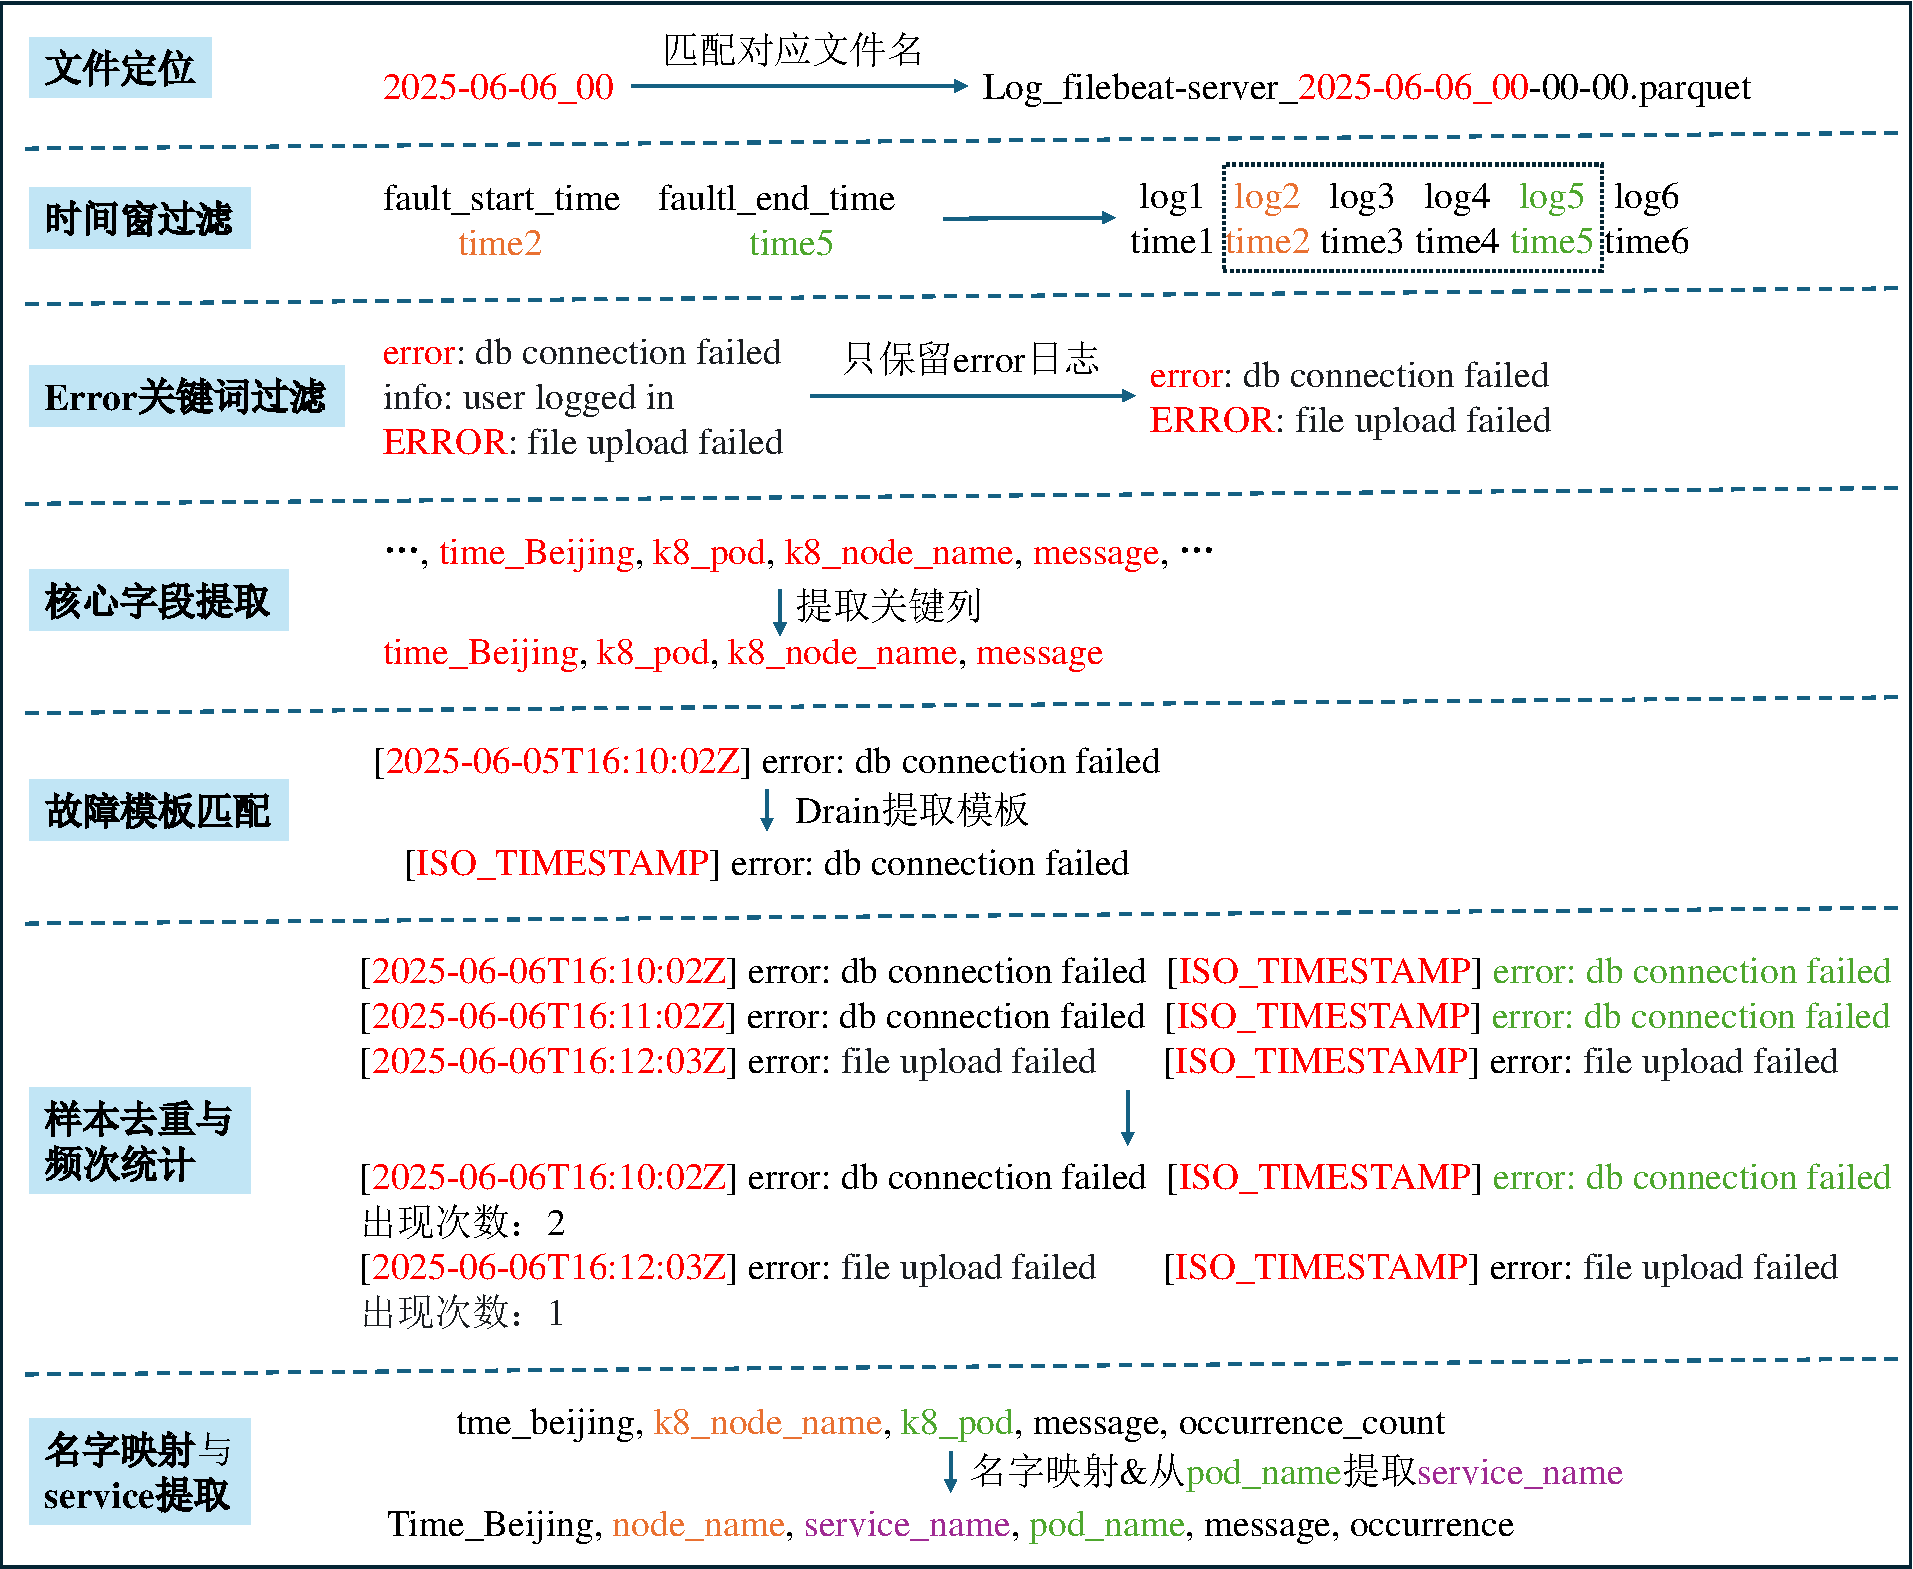
\includegraphics[width=0.95\textwidth]{pics/fig6.pdf}
    \caption{多层级数据筛选处理流程}
    \label{fig6}
\end{figure*}

\subsection{数据预处理}
\label{sec:data-preprocess}

数据预处理模块聚焦于输入数据解析和多模态时间戳统一处理两个核心功能,确保后续各模态数据处理的一致性和准确性,为整个故障根因定位系统奠定数据基础。

\subsubsection{输入数据解析设计}
\label{sec:input-data-parse}

输入数据采用基于正则表达式的提取策略,对原始故障描述文件进行结构化处理。系统接收包含故障描述(Anomaly Description)和唯一标识符(uuid)的JSON格式输入数据,其中最关键的信息是故障描述中的故障起止时间和uuid。

为便于后续多模态数据的精准匹配和故障时间段数据筛选,系统首先对输入文件进行关键信息解析提取,核心包括故障唯一标识和故障起止时间等,如\ref{fig2}所示。

\textbf{时间戳提取机制:}系统采用ISO 8601时间格式标准,通过正则表达式模式 \verb!(\d{4}-\d{2}-\d{2}T\d{2}:\d{2}:\d{2}Z)! 实现自动化时间戳识别。提取规则遵循“首个匹配为故障起始时间,次个匹配为故障结束时间”的策略。

\textbf{时间索引生成:}为提升后续数据关联效率,系统构建了多层级时间索引机制。生成“年-月-日\_时”格式的时间标识(如2025-06-06\_00),用于快速定位对应的数据文件。同时将故障时间转换为19位纳秒级时间戳,为精确的时间范围筛选提供高精度基准,预处理后的input数据具体如\ref{fig3}所示。

\subsubsection{多模态数据时间戳统一}
\label{sec:multi-modal-timestamp-unify}

针对log、 trace和metric三种数据的不同格式特点,系统地设计了差异化的时间戳统一处理策略,实现跨模态时间基准的标准化,具体如\ref{fig4}所示。

\textbf{Log数据时间戳标准化:}log数据采用ISO 8601格式的@timestamp字段作为时间基准。系统通过时间格式解析,将原始时间戳转换为统一的19位纳秒级时间戳。处理完成后按时间戳升序排列,确保数据的时序一致性和后续分析的准确性。

\textbf{Metric数据时间戳处理:}metric数据使用time字段存储时间信息,同样遵循ISO 8601格式标准。考虑到metric数据在存储架构中的多层级分布特点,系统采用递归搜索策略,遍历所有子目录结构,确保完整覆盖分散存储的指标文件。时间戳转换逻辑与日志数据保持一致。

\textbf{Trace数据时间戳转换:}trace数据具有独特的时间存储格式,使用startTime字段存储微秒级时间戳。本文通过精度转换,将微秒级时间戳扩展为纳秒级(乘以1000倍数),实现与其他模态数据的时间精度对齐。

\subsection{Log故障抽取}
\label{sec:log-fault-extraction}

日志故障抽取模块是故障根因定位系统的核心组件,采用多层级筛选策略,可将海量原始日志高效转换为结构化故障特征信息。该模块的故障信息压缩功能基于预训练的Drain算法模型,通过提取error字段日志的模板,并对同一模板的日志进行去重处理,实现对故障日志的有效压缩,从而为后续的多模态故障分析提供高质量的结构化log数据输入。

\subsubsection{日志解析原理与模型构建}
\label{sec:log-parse-principle-and-model-build}

\paragraph{非结构化日志处理挑战}

系统日志作为非结构化信息载体,详细记录了系统的操作行为,但同时包含大量影响分析效率的无关变量(如时间戳、IP地址、端口号等)。这些变量在日志中虽有重要意义,但在故障模式识别过程中,容易导致大量语义相同但表现形式不同的重复记录。这些重复记录占用了宝贵的大语言模型上下文空间,却无法提供额外的有效信息。

\paragraph{Drain算法选择与应用}

经过对现有日志解析技术的综合评估,本研究采用广泛认可的Drain算法作为核心日志解析器。Drain算法通过构建解析树的方式,能够有效识别日志中的固定部分和可变部分,将具有相同语义模式的日志归类为同一模板。这一过程实现了从非结构化日志到结构化特征的转换,同时压缩了大量冗余的日志。具体而言,Drain算法提取日志的模板,并去除无关变量(时间、id等),将相同模板的日志合并为一个条目,从而有效减少数据量。\ref{fig5}展示了日志模板的提取操作,其输出中所有的变量都由Drain解析成不变的内容,能减少无关变量的干扰。

\paragraph{预训练模型构建}

系统基于phaseone中的全量日志数据,筛选出所有包含error字段的日志记录作为训练样本,构建Drain预训练模型。通过对微服务环境中海量错误日志的学习分析,模型成功提取并构建了156个具有代表性的故障模板,较为全面的覆盖了微服务系统中的主要故障模式类型。

\subsubsection{多层级数据筛选处理流程}

多层级数据筛选处理流程具体如\ref{fig6}所示,从文件定位开始,经时间窗过滤、error关键词过滤、核心字段提取与重构、故障模板匹配、样本去重与频次统计,到名字映射与service提取。最终将海量日志转化为结构化故障特征,同时实现有效的内容压缩。

\paragraph{文件定位}

系统根据预处理部分输出的每项input时间信息,采用“年-月-日\_时”格式的时间标识进行文件匹配,如\ref{fig7}所示。通过在项目数据目录中搜索对应时间段的日志文件,确保精准定位到故障时间窗口内的数据源。

\begin{figure*}[htbp]
    \centering
    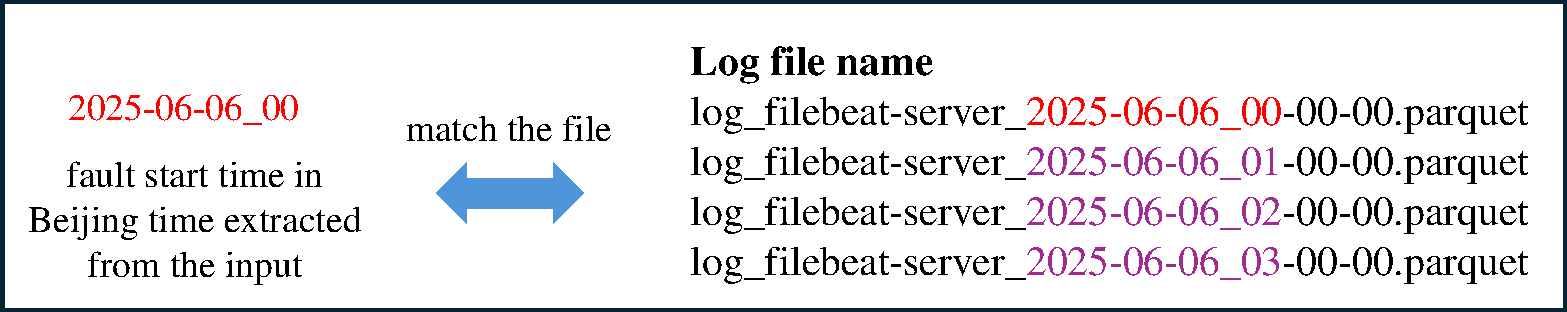
\includegraphics[width=0.95\textwidth]{pics/fig7.pdf}
    \caption{input 中的时间与 log 文件名匹配}
    \label{fig7}
\end{figure*}

\paragraph{时间窗过滤}

基于故障起止时间的纳秒级精度时间戳,对日志数据执行严格的时间边界筛选。系统通过时间戳字段进行范围查询,确保仅保留故障时间段内的日志记录,有效排除时间维度上的无关信息干扰。

\paragraph{Error 关键词过滤}

针对日志消息字段实施基于“error”关键词的过滤机制。在进行大量日志数据分析后,观察到故障可能伴随error字段的形式大量出现,因此,自动识别和提取包含error信息的日志条目,过滤掉正常业务操作日志,从而显著提升后续分析的针对性和效率。

\paragraph{核心字段提取与重构}

从原始日志的多维度字段中精确提取分析必需的核心信息,包括时间信息(time\_beijing)、容器标识(k8\_pod)、节点信息 (k8\_node\_name) 和错误消息内容 (message) 等关键维度。通过字段精简策略减少数据冗余,同时保证信息完整性。

\paragraph{故障模板匹配与标准化}

利用预训练的Drain模型对每条错误日志进行模板匹配。系统将原始日志消息转换为标准化的模板表示形式,去除无关变量,仅保留核心故障语义内容,实现从个体日志到模式类别的提取。

\paragraph{样本去重与频次统计}

针对相同容器和模板组合的重复日志记录(比如:[[2025-06-06 08:00, \textbf{frontend-0}, \textbf{template0}, message0], [2025-06-06 09:00, \textbf{frontend-0}, \textbf{template0}, message1]]),采用去重策略。系统保留每种组合的首次出现记录,同时统计该组合的出现频次[2025-06-06 08:00, frontend-0, message0, 出现次数: 2],通过量化标注为故障严重程度评估提供客观依据。

\paragraph{名字映射与service提取}

Log中的k8\_node\_name和k8\_pod进行映射,转换为node\_name和pod\_name,并通过解析pod\_name提取对应的service信息(例如:frontend-0→frontend)。最终,系统将数据重构为标准化的多层次格式,包含node、service、pod、错误消息和频次统计等维度,为后续的多模态故障分析提供结构化的数据基础。

通过上述系统化的处理流程,log故障抽取模块能够将原始的海量日志数据高效压缩为高质量的结构化故障特征集合,最终抽取出来的故障示例具体如\ref{fig8}所示。该模块不仅显著降低了数据处理复杂度,还保持了故障信息的完整性和准确性,为后续基于智能体的多模态故障根因定位提供log层次的数据基础。

\begin{figure*}[htbp]
    \centering
    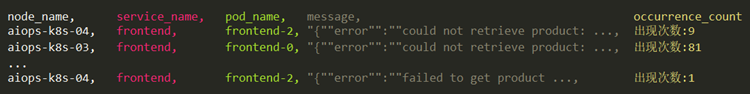
\includegraphics[width=0.95\textwidth]{pics/fig8.png}
    \caption{log 故障抽取输出}
    \label{fig8}
\end{figure*}

\subsection{Trace 故障检测}

调用链故障检测模块是微服务系统故障根因定位的关键组件,采用双重异常检测策略,分别从性能维度和状态维度识别微服务调用链中的异常模式。该模块基于IsolationForest机器学习算法和状态码直接检查方法,实现对duration异常和status异常的有效识别,两种识别结果同时传入多模态分析,为后续的多模态故障分析提供高质量的结构化trace数据输入。

\subsubsection{双重异常检测原理与模型构建}

微服务架构下的分布式调用链包含丰富的性能和状态信息,但异常模式呈现多样化特征。性能异常主要表现为调用链duration的明显偏离正常范围,需要通过机器学习方法建立正常行为基线;状态异常则体现为明显的错误码出现,可通过直接检查的方式识别。两种异常检测机制的结合能够提供更丰富的故障特征信息。

\paragraph{IsolationForest 性能异常检测原理}

针对duration性能异常检测,采用IsolationForest无监督学习算法。该算法基于“异常点在特征空间中更容易被孤立”的核心假设,通过构建多个随机分割树来量化数据点的异常程度。IsolationForest特别适用于连续数值型数据的异常检测,能够在不需要标注异常样本的情况下,自动识别duration数据中的明显偏离模式。

\paragraph{状态码直接检查机制}

并行构建基于状态码的直接检查机制,无需训练过程。系统直接分析trace数据中tags中的status.code和status.message字段,通过简单的条件判断(status.code≠0)筛选出所有异常状态调用。这种方法能够直接捕获系统错误、超时、连接失败等明确的异常状态和具体信息,为故障根因定位提供确定性的异常证据。

\paragraph{IsolationForest 训练数据构建与模型训练}

\begin{figure*}[htbp]
    \centering
    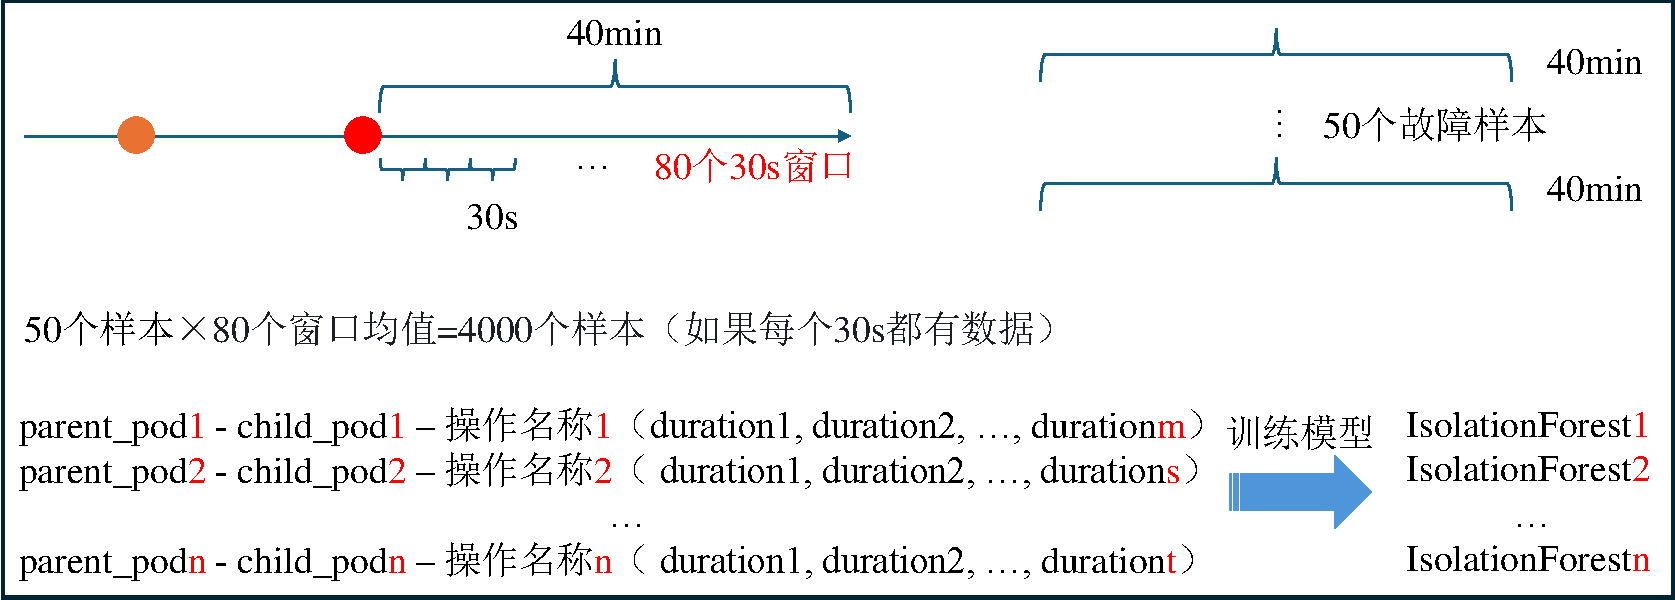
\includegraphics[width=0.95\textwidth]{pics/fig9.pdf}
    \caption{IsolationForest 训练数据构建与模型训练}
    \label{fig9}
\end{figure*}

IsolationForest训练数据构建与模型训练如\ref{fig9}所示,主要包括下面几部分内容:

\textbf{训练数据来源:}本方案利用phaseone阶段的数据构建训练集。通过随机抽样50个故障样本,提取每个故障结束后40分钟的时间窗口作为“正常时期”数据。这种基于故障恢复后系统行为趋于正常的假设,确保了大部分训练数据都是正常数据。

\textbf{分组训练策略:}按照“parent\_pod - child\_pod - 操作名称”的服务调用组合对训练数据进行分组,为每个唯一的服务调用模式训练独立的IsolationForest检测器。这种细粒度的分组策略考虑了不同服务调用的性能基线差异,提升了异常检测的精准度。

\textbf{滑动窗口平均化处理:}在训练阶段,采用30秒滑动窗口对duration数据进行事件序列处理。由于一个30秒滑动窗口内可能出现多种“parent\_pod - child\_pod - 操作名称”的调用组合,且每种组合可能出现一次或多次,因此针对窗口内同一种组合,若出现一次及以上,则计算器duration的平均值;若未出现,则记为None。这种处理方式能有效消除单个调用样本的随机波动,让duration特征更稳定,从而更准确地反映服务调用的真实性能水平。

\textbf{异常检测阈值设置:}IsolationForest模型采用contamination参数设置为0.01(即预期异常样本占总体的1\%),同时使用n\_estimators=100构建100个决策树。模型输出异常分数,当分数为-1时判定为异常,为1时判定为正常。

\subsubsection{多维度 trace 数据处理流程}

\paragraph{文件定位与时间过滤}

系统根据预处理部分解析出的每项input时间信息,采用“年-月-日\_时”格式进行trace文件精确匹配。基于故障起止时间的纳秒级时间戳,对调用链数据执行时间窗口筛选,确保分析范围覆盖完整的故障时间段。

\paragraph{调用关系映射与结构化提取}

从复杂的trace结构中提取关键维度信息,包括通过解析process字段获取pod\_name、service\_name、node\_name,利用spanID和references建立完整的调用链父子关系映射。系统将非结构化trace数据转换为包含“parent\_pod - child\_pod - 操作名称”调用表示。

\paragraph{Duration 异常检测处理流程}


\textbf{预测数据处理:}对故障时间段内的所有trace数据进行异常检测预测,采用与训练阶段相同的30秒滑动窗口策略,计算每个时间窗口内的duration平均值。这种一致性处理确保了训练和预测阶段的特征分布一致性。

\textbf{IsolationForest异常预测:}利用预训练的检测模型对故障期间的duration特征进行异常识别。每个服务调用组合使用对应的专用检测器进行预测(若故障期间存在之前未训练的调用组合则忽略不进行预测),输出异常标签(-1表示异常,1表示正常)。

\textbf{Duration异常结果输出:}系统输出前20个最频繁的duration异常组合,包含以下具体内容:

\begin{itemize}
    \item node\_name:异常发生的节点标识;
    \item service\_name:异常服务名称;
    \item parent\_pod:调用方容器标识;
    \item child\_pod:被调用方容器标识;
    \item operation\_name:具体操作名称;
    \item normal\_avg\_duration:正常时期的平均调用时延(来自训练数据统计);
    \item anomaly\_avg\_duration:异常时期的平均调用时延(来自故障阶段实际统计);
    \item anomaly\_count:异常出现频次(格式:出现次数:N);
\end{itemize}

\begin{figure*}[htbp]
    \centering
    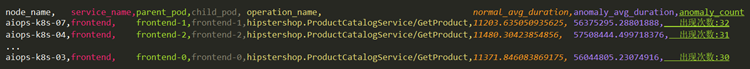
\includegraphics[width=0.95\textwidth]{pics/fig10.png}
    \caption{IsolationForest 检测出来的异常 trace 示例输出}
    \label{fig10}
\end{figure*}

利用IsolationForest检测得到的异常trace的具体输出实例如\ref{fig10}所示。

\paragraph{Status 状态异常检测处理流程}

\textbf{直接状态检查:}对故障时间段内的所有trace数据进行状态码检查,无需训练过程。从trace的tags字段中解析status.code和status.message信息,通过条件过滤(status.code≠0)直接识别所有异常状态调用。

\textbf{状态异常模式统计:}对识别出的状态异常按照服务调用组合进行分组统计,计算每种异常模式的出现频次。

\textbf{Status状态结果输出:}系统输出前20个最频繁的状态异常组合,包含以下具体内容:

\begin{itemize}
    \item Node\_name:异常发生的节点标识;
    \item Service\_name:异常服务名称(redis自动映射为redis-cart);
    \item Parent\_pod:调用方容器标识;
    \item Child\_pod:被调用方容器标识;
    \item Operation\_name:具体操作名称;
    \item Status\_code:具体的错误状态码;
    \item Status\_message:错误状态的详细描述信息;
    \item Occurrence\_count:状态异常出现频次(格式:出现次数:N);
\end{itemize}

\begin{figure*}[htbp]
    \centering
    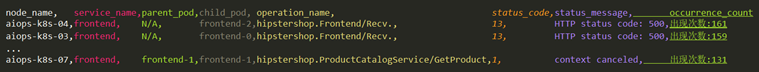
\includegraphics[width=0.95\textwidth]{pics/fig11.png}
    \caption{status 状态检测出来的异常 trace 示例输出}
    \label{fig11}
\end{figure*}

利用status状态检测得到的异常trace具体输出实例如\ref{fig11}所示。

通过上述双重异常检测流程,trace故障检测模块实现了基于机器学习的异常识别和基于规则的直接异常检查的有机结合。Duration异常检测通过IsolationForest算法提供量化的性能异常分析,status异常检测通过直接检查提供确定性的错误状态识别。两种检测策略分别输出的前20个最重要的异常模式,为后续故障根因定位提供trace数据基础。

\subsection{Metric 故障总结}

指标故障总结模块是分布式微服务系统故障的全栈监控分析组件,采用基于大语言模型的双层级现象总结策略(见\ref{fig12}),通过规则筛选和统计对比方法识别显著异常指标,利用大模型的推理能力对复杂的多为监控数据进行现象归纳和模式识别,为后续的多模态故障根因分析提供高质量的现象描述输入。

\begin{figure}[htbp]
    \centering
    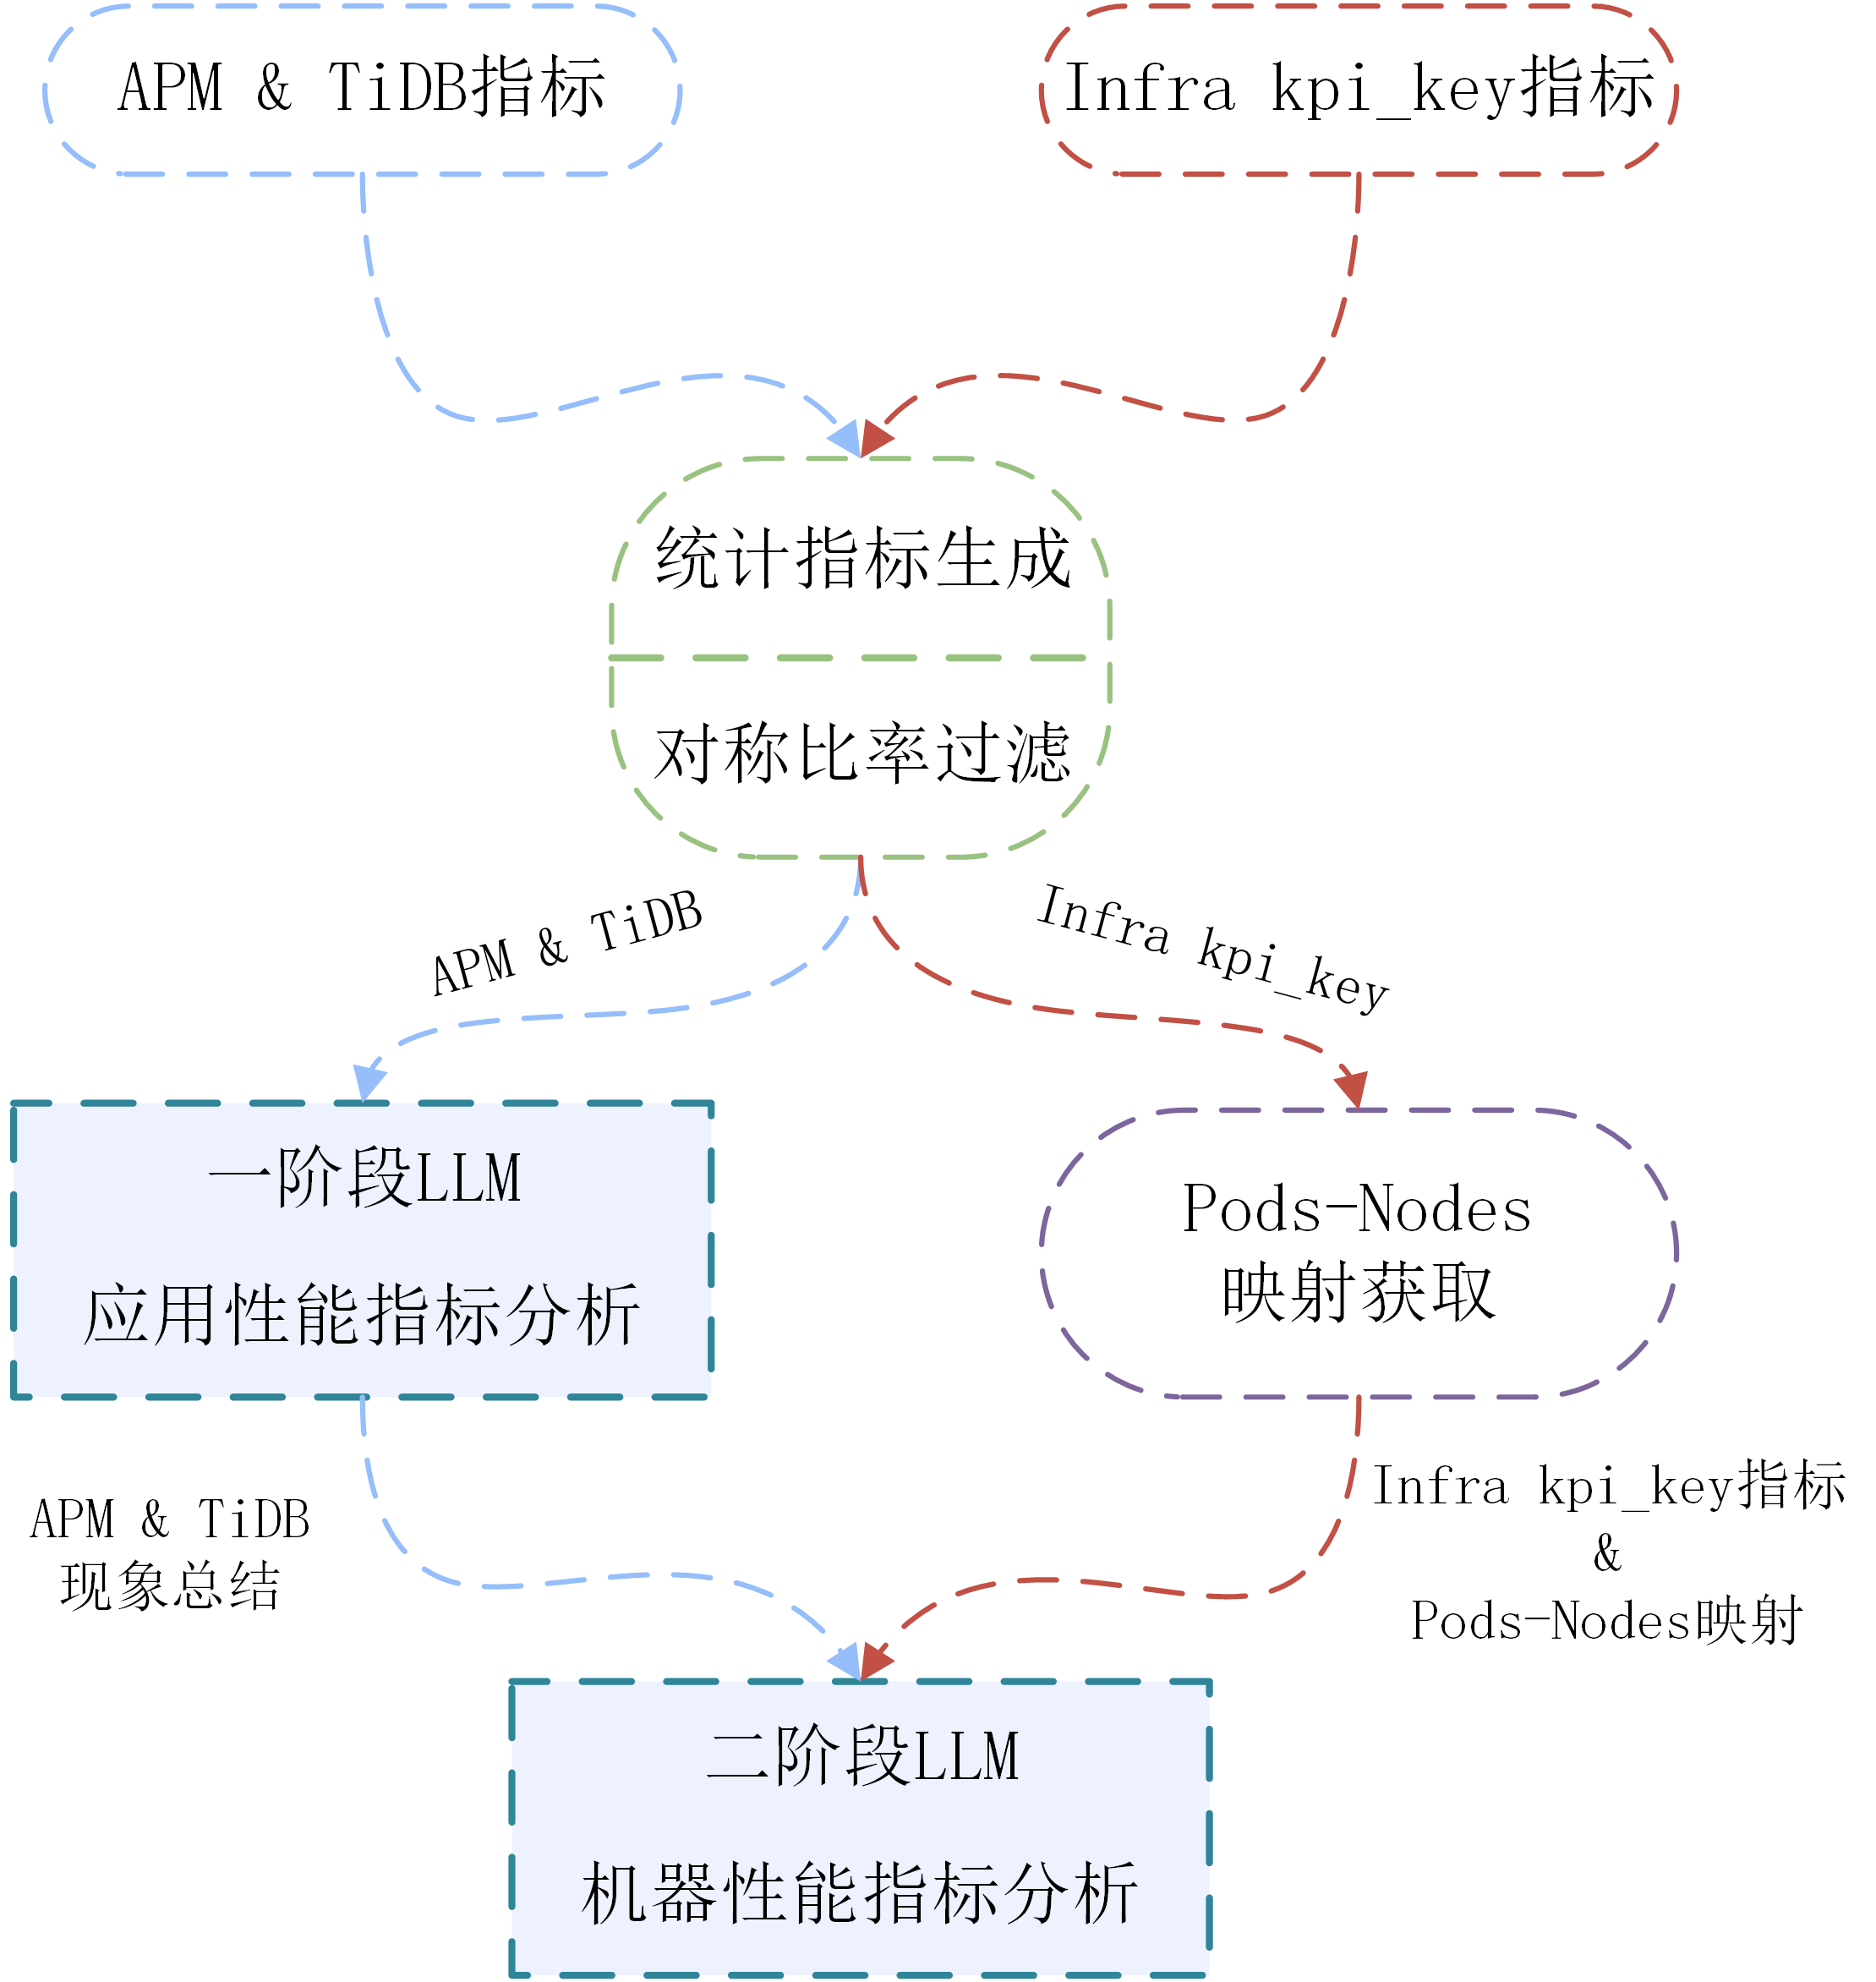
\includegraphics[width=0.45\textwidth]{pics/fig12.png}
    \caption{双层级大模型现象总结示意图}
    \label{fig12}
\end{figure}

\subsubsection{大模型驱动的现象总结原理与方法构建}

\paragraph{传统异常检测方法的局限性}

分布式微服务架构下的监控指标具有高维度、多层次和强关联的特征,传统的基于阈值或机器学习的异常检测方法往往只能识别单一指标的数值异常,难以理解指标间的关联关系和业务语义。这些方法缺乏对异常现象的语义化描述能力,无法为后续的多模态故障根因定位提供可解释的现象总结。

\paragraph{大模型现象总结方法}

本方案在metric数据处理方法中,采用大语言模型作为核心的现象总结工具,充分利用其强大的语义理解和推理归纳能力。通过传递筛选出来的监控数据,让模型自动识别异常变化模式、关联关系和业务影响,输出语义丰富的现象描述。需要特别强调的是,本模块的大模型仅用于现象总结和模式描述,不进行故障判断或根因推断,为后续结合log和trace等多模态数据的综合根因分析奠定基础。

\paragraph{正常时间段定义}

系统采用相对时间窗口的方式定义正常时间段,具体规则为:提取当前故障前一个故障结束后10分钟至当前故障开始前的时间段,以及当前故障结束后10分钟至下一个故障开始前的时间段作为正常运行时间段。这种定义方式不仅确保正常时间段数据反映微服务系统的稳定运行状态,避免了故障“余波”影响的干扰,还通过选择故障时间段前后的相邻时间窗口,有效减少了每日不同时间段业务波动的影响(如白天访问量高峰与夜间访问量低估),为对比分析提供更加可靠的性能基线。

\subsubsection{多层级监控指标体系与筛选}

\paragraph{Pod-Service 统一分析架构}

所提出系统将pod和service层级进行统一处理,通过解析Pod名称自动提取Service标识。例如frontend-0、frontend-1、frontend-2等Pod实例通过去除数字后缀统一归类为frontend服务。这种设计简化了微服务架构下的分析复杂度,同时保持了服务级别和实例级别的双重视角,能够有效识别服务级别的共性问题和个别实例的特异性异常。

\paragraph{应用性能监控指标筛选}

从微服务APM监控数据的众多冗余指标中精选出7个核心关键指标:client\_error\_ratio(客户端错误率)、error\_ratio(总体错误率)、request(请求数量)、response(响应数量)、rrt(平均响应时间)、server\_error\_ratio(服务端错误率)、timeout(超时次数)。这些指标涵盖了微服务性能的核心维度,能够全面反映服务的健康状况和异常特征,同时避免了冗余数据对现象分析效果的影响。

\paragraph{机器性能指标监控指标分层覆盖}

构建涵盖容器层和节点层的基础设施监控体系。容器层包含9个Pod基础设施指标:pod\_cpu\_usage(pod CPU使用率)、pod\_memory\_working\_set\_bytes(pod工作集内存使用量)、pod\_fs\_reads\_bytes(pod文件系统读取字节数)、pod\_fs\_writes\_bytes(pod文件系统写入字节数)、pod\_network\_receive\_bytes(pod网络接收字节数)、pod\_network\_receive\_packets(pod网络接收数据包数)、pod\_network\_transmit\_bytes(pod网络发送字节数)、pod\_network\_transmit\_packets(pod网络发送数据包数)、pod\_processes(pod内运行进程数量)。节点层包含16个Node基础设施指标:node\_cpu\_usage\_rate(节点CPU使用率)、node\_memory\_usage\_rate(节点内存使用率)、node\_disk\_read\_bytes\_total(磁盘读取字节数)、node\_disk\_written\_bytes\_total(磁盘写入字节数)、node\_disk\_read\_time\_seconds\_total(磁盘读取时间)、node\_disk\_write\_time\_seconds\_total(磁盘写入时间)、node\_filesystem\_usage\_rate(文件系统使用率)、node\_network\_receive\_bytes\_total(网络接收字节数)、node\_network\_transmit\_bytes\_total(网络发送字节数)、node\_network\_receive\_packets\_total(网络接收数据包总数)、node\_network\_transmit\_packets\_total(网络发送数据包总数)、node\_sockstat\_TCP\_inuse(TCP连接数)等。通过分层监控确保从微服务应用到具体部署的基础机器设施的完整覆盖。

\paragraph{TiDB 数据库组件监控指标}

针对TiDB分布式数据库构建专项监控指标体系,覆盖tidb-tidb、tidb-tikv、tidb-pd三个核心组件。包括failed\_query\_ops(失败查询数)、duration\_99th(99分位请求延迟)、connection\_count(连接数)、server\_is\_up(服务存活节点数)、cpu\_usage(CPU使用率)、memory\_usage(内存使用量)、store\_up\_count(健康Store数量)、store\_down\_count(Down Store数量)、store\_unhealth\_count(不健康Store数量)、storage\_used\_ratio(已用容量比)、available\_size(可用存储容量)、raft\_propose\_wait(RaftPropose等待延迟)、raft\_apply\_wait(RaftApply等待延迟)、rocksdb\_write\_stall(RocksDB写阻塞次数)等数据库特有指标,实现对数据存储层的专业化监控分析。

\subsubsection{数据处理与异常筛选流程}

\paragraph{分层级数据加载与组织}

系统根据预处理部分输出的每项input日期信息,按照监控层级构建不同的数据路径进行文件定位。APM业务监控数据位于“年-月-日/metric-parquet/apm/pod”目录,基础设施节点监控数据位于“年-月-日/metric-parquet/infra/infra\_node”目录,容器监控数据位于“年-月-日/metric-parquet/infra/infra\_pod”目录,TiDB数据库监控数据位于“年-月-日/metric-parquet/infra/infra\_tidb”等目录。通过分层级的文件组织方式安监控维度进行精准的数据定位和加载。

\paragraph{时间窗口精准过滤与数据合并}

系统对各层级监控数据执行纳秒级时间窗口筛选,确保分析范围完整覆盖故障时间段。将故障时间段前后2个正常时间段的数据进行合并处理,跳过故障时间段前10分钟,以消除故障“余波”造成的影响,并通过移除最大最小各2个极值的方式消除随机波动影响,构建稳定的统计基线。这种处理方式确保正常期间数据的代表性和稳定性。

\paragraph{基于统计对称比率的显著性筛选}

实施基于统计对称比率的显著性筛选机制,计算故障期间与正常期间的中位数和99分位数的对称比率。自动过滤变化幅度小于5\%的稳定指标,仅保留变化显著的可能关键异常指标进入大模型分析流程。这种筛选策略能够将海量原始数据压缩为高价值的异常特征集合,大幅度减少大模型的上下文,token数量减少50\%左右,同时显著提升现象总结的效率和质量,以P50的对称比率为例,其具体公式定义如下:

\begin{equation}
P50_{\mathrm{symmetric\text{-}ratio}} = \frac{ \left| P50_{\mathrm{fault}} - P50_{\mathrm{normal}} \right| }{ \frac{ P50_{\mathrm{fault}} + P50_{\mathrm{normal}} }{2} + \varepsilon }
\end{equation}

其中 $P50$ 表示中位数,$P50_{\mathrm{fault}}$ 和 $P50_{\mathrm{normal}}$ 分别为故障期间和正常期间的中位数,$\varepsilon$ 为极小值。

对筛选后的关键指标,利用pandas的describe方法提取完整的描述统计信息,包括中位数、四分位距、99分位数等关键统计量。通过标准化的数据表示格式,将不同类型和量纲的监控指标转换为大模型可理解的结构化输入,确保后续现象总结的准确性和一致性。

\subsubsection{双层级大模型现象总结与输出生成}

\paragraph{第一层:应用性能监控现象识别与总结}

系统首先对微服务应用性能监控指标和TiDB数据库组件指标进行综合分析。将筛选后的关键异常指标按服务类型组织、每个服务包含其下属多个Pod实例数据。例如emailservice服务包含emailservice-0、emailservice-1、emailservice-2等多个pod实例的client\_error\_ratio(客户端错误率)、error\_ratio(总体错误率)、request(请求数量)、response(响应数量)、rrt(平均响应时间)、server\_error\_ratio(服务端错误率)、timeout(超时次数)等APM指标对比数据。同时整合TiDB各组件的failed\_query\_ops(失败查询数)、duration\_99th(99分位请求延迟)、connection\_count(连接数)等数据库专项指标。构建包含正常期间和故障期间对比数据的结构化表格,通过service-pod的层次化组织方式,调用大语言模型进行第一次现象总结,提示词设计见\ref{fig13},数据对比表格采用json形式,与markdown形式相比,json格式在保持清晰度的同时,大幅度减少token使用量,具体形式如\ref{fig14}所示。在分析pod级别现象的同时,自然总结出服务级别的共性现象和差异化表现。此阶段大模型仅进行现象描述,不做故障判断。

\begin{figure*}[htbp]
    \centering
    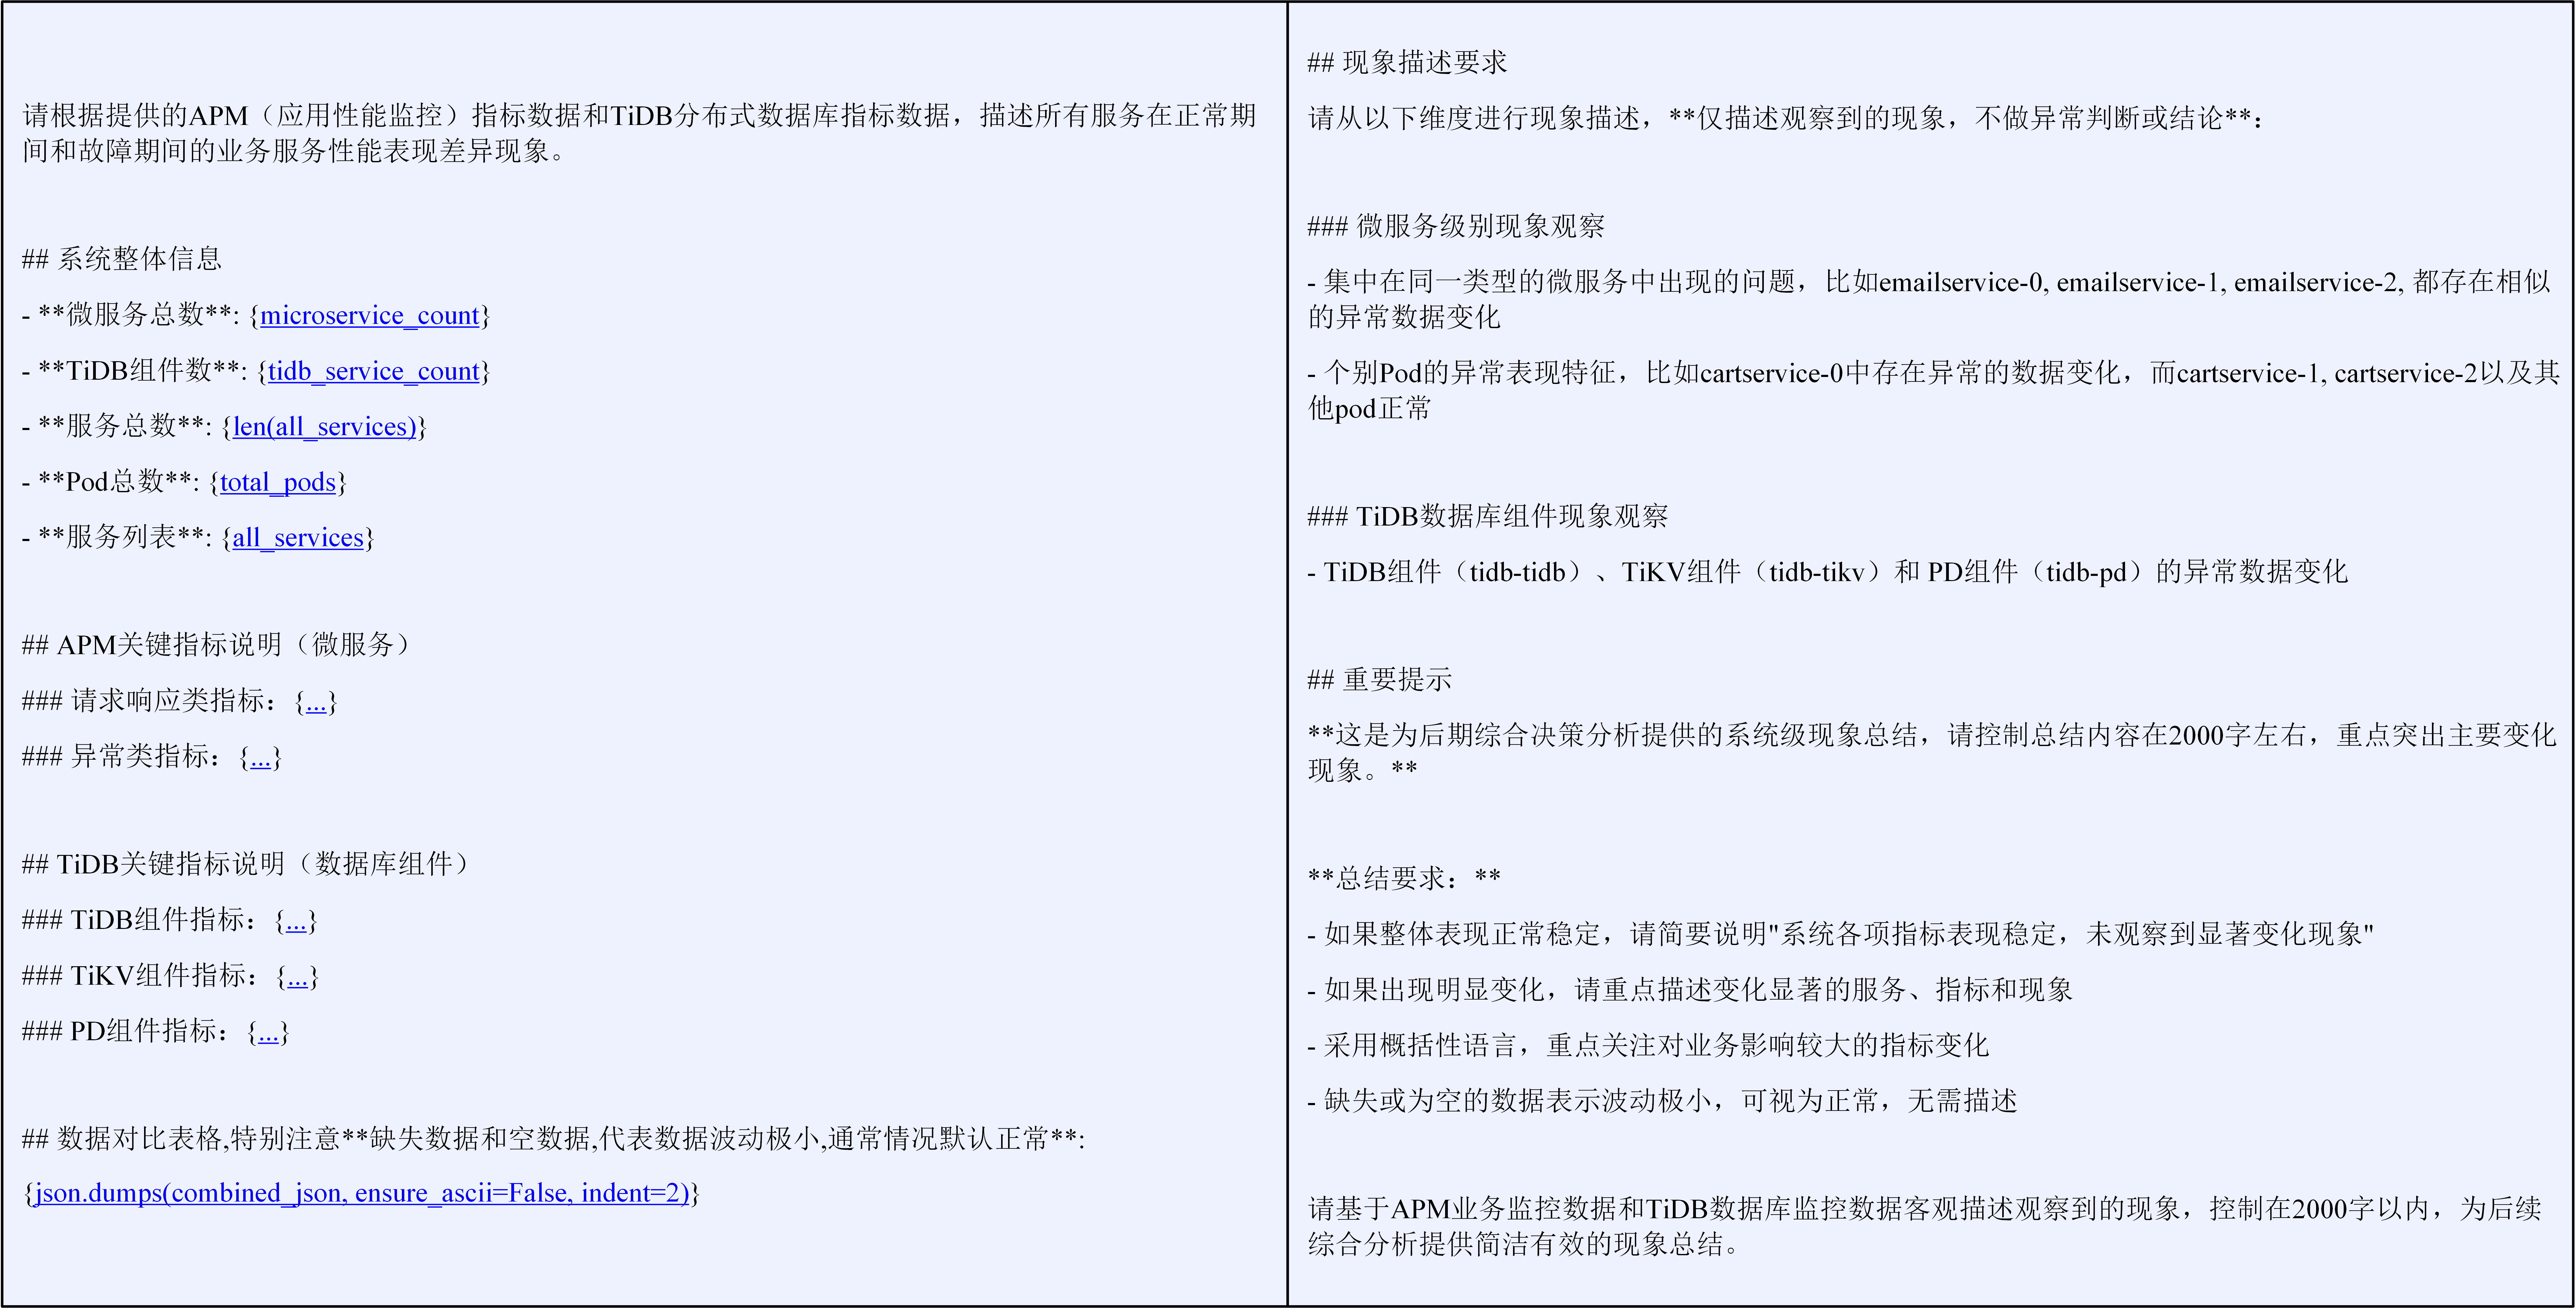
\includegraphics[width=0.95\textwidth]{pics/fig13.png}
    \caption{业务指标和 TiDB 数据库组件指标综合分析 prompt}
    \label{fig13}
\end{figure*}

\begin{figure*}[htbp]
    \centering
    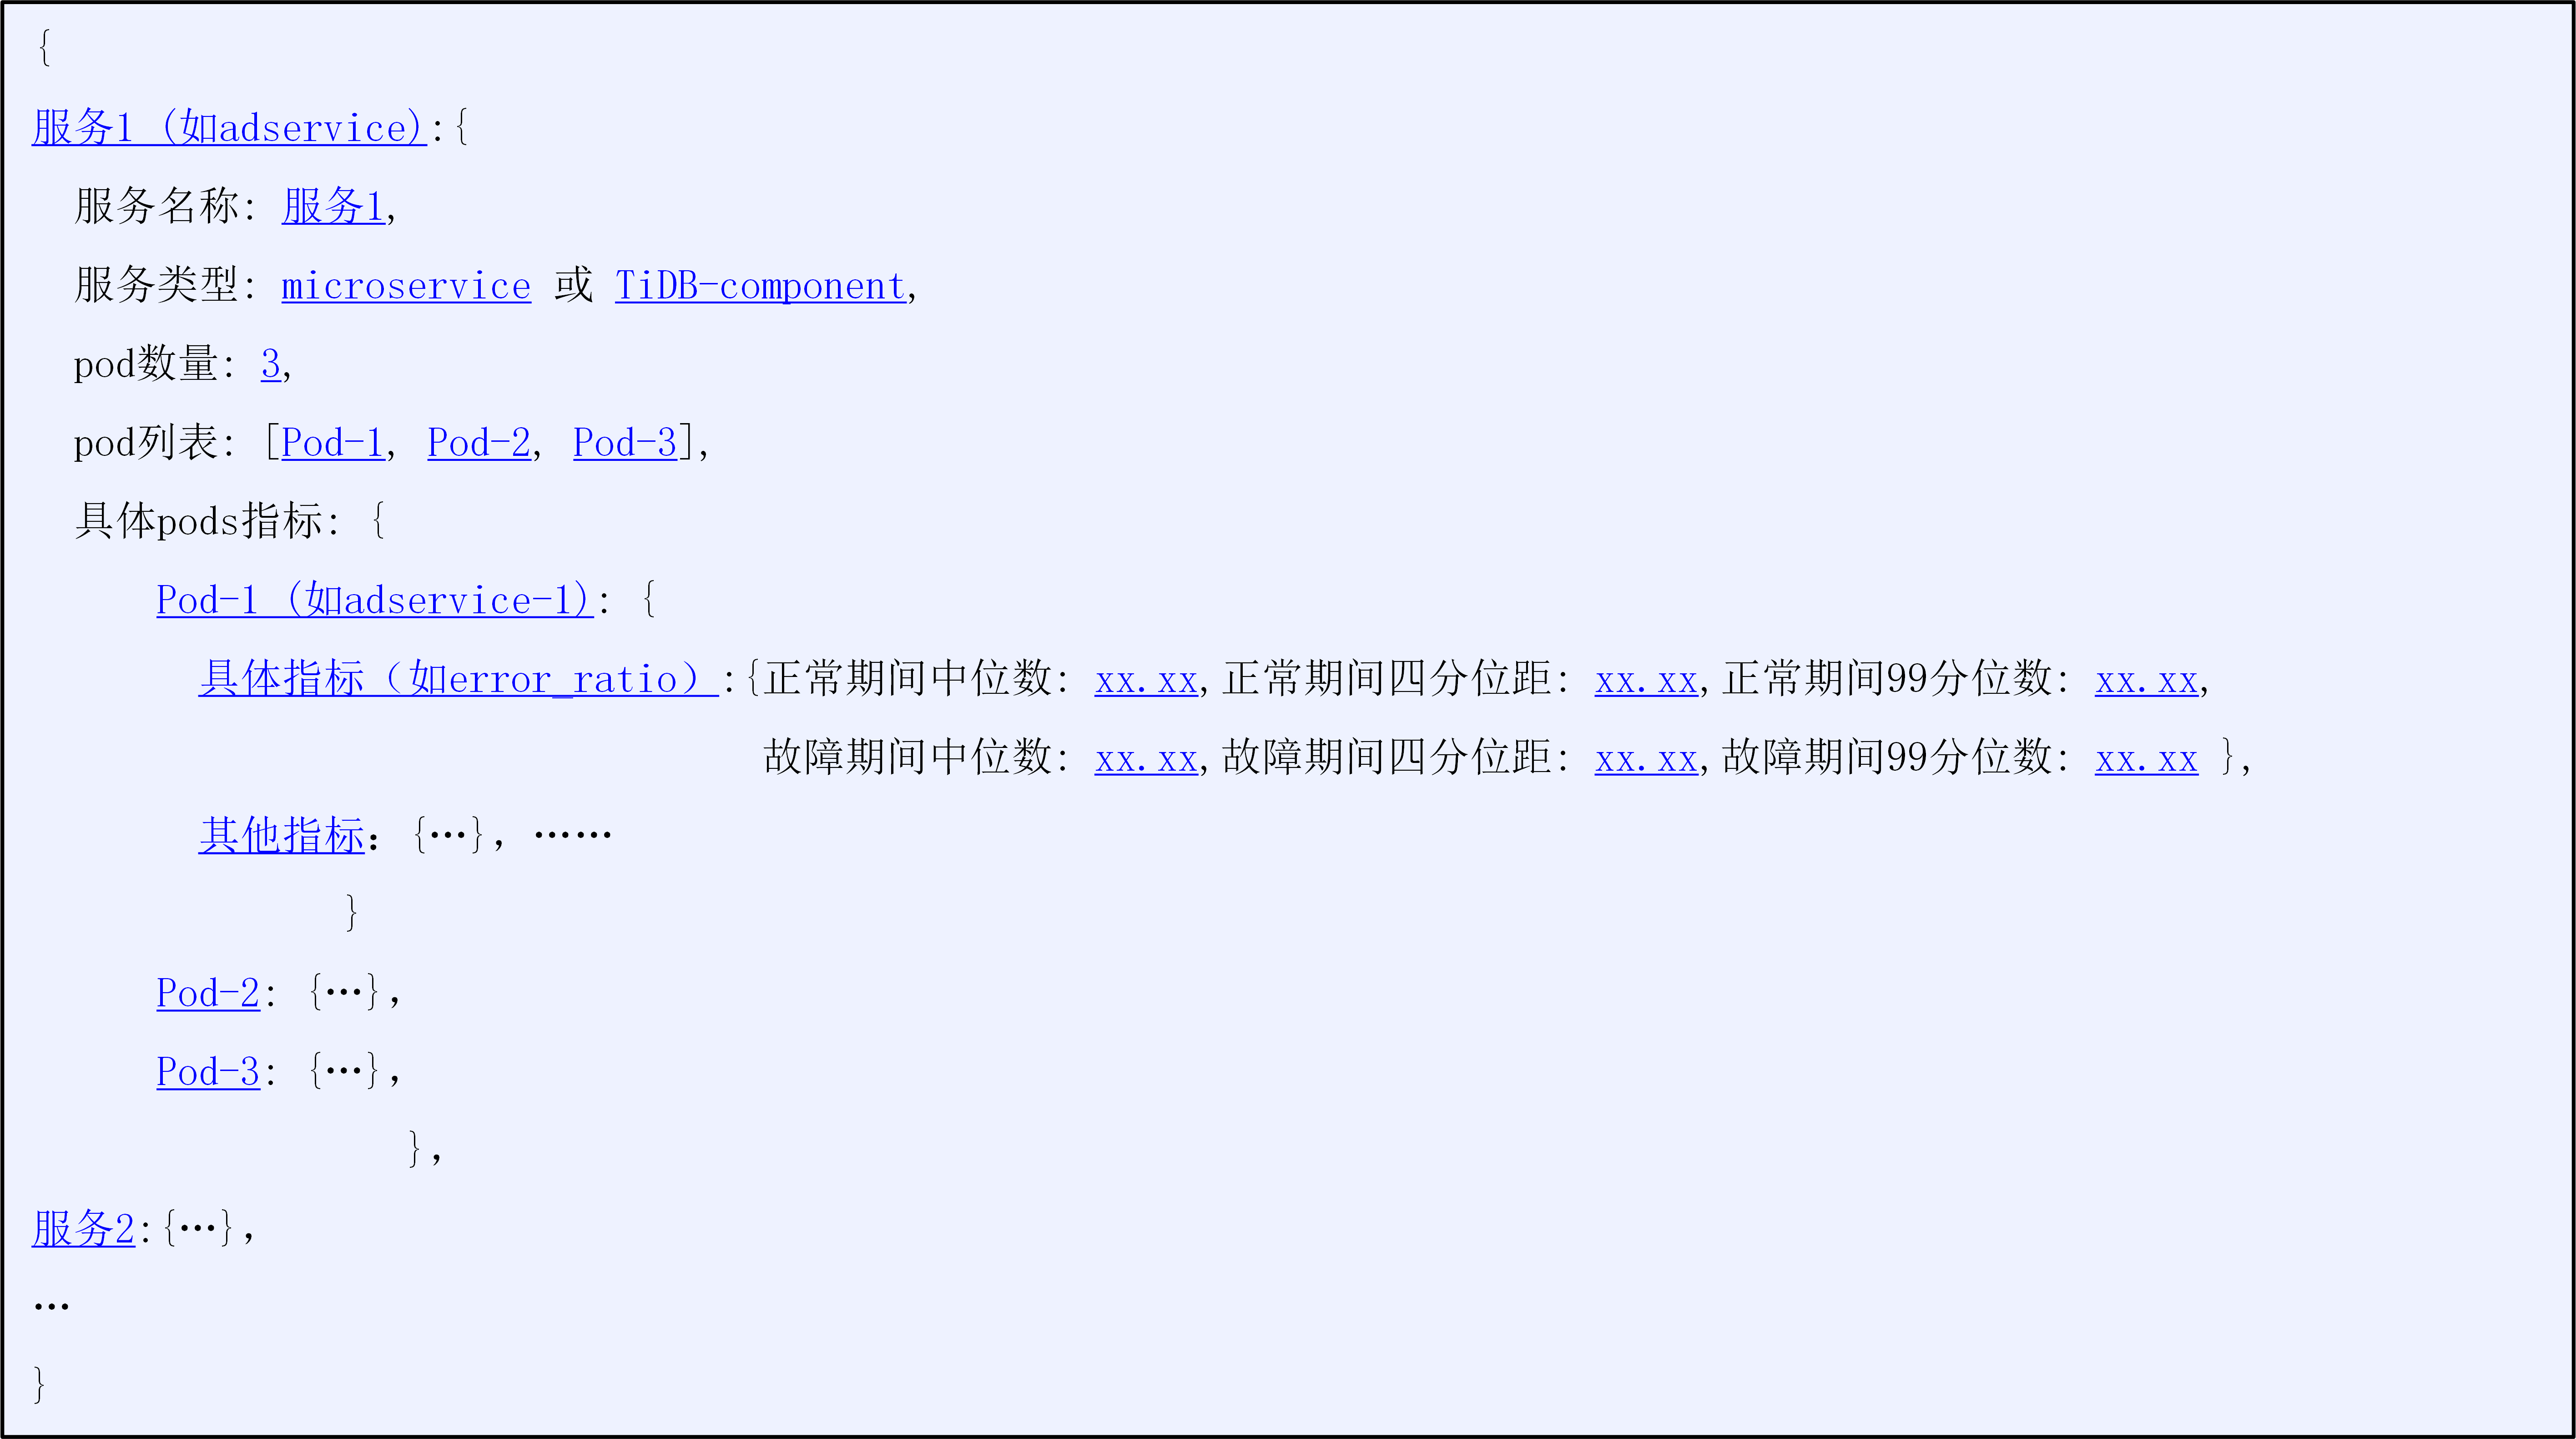
\includegraphics[width=0.95\textwidth]{pics/fig14.png}
    \caption{业务指标和 TiDB 数据库组件对比数据示例}
    \label{fig14}
\end{figure*}

\paragraph{第二层:基础设施机器性能指标综合现象总结与关联分析}

在应用性能监控数据的分析基础上,系统进一步整合pod容器层和node节点层的基础设施的机器性能监控数据。结合pod在各节点的部署拓扑信息和第一层的服务分析结果,构建涵盖应用、容器、节点三个层级的全栈现象视图。整合pod\_cpu\_usage(Pod CPU使用率)、pod\_memory\_working\_set\_bytes(Pod工作集内存使用量)、pod\_network\_receive\_bytes(Pod网络接收字节数)等容器指标,以及node\_cpu\_usage\_rate(节点CPU使用率)、node\_memory\_usage\_rate(节点内存使用率)、node\_disk\_read\_bytes\_total(磁盘读取字节数)、node\_network\_transmit\_bytes\_total(网络发送字节数)等节点指标。调用大语言模型进行第二次综合现象总结,数据对比表格同样采用json形式,在描述节点kpi\_key统计指标后,描述在此节点上部署的pods相关kpi\_key指标,以保持紧密的数据流,具体形式如\ref{fig15}所示,提示词设计如\ref{fig16}所示。重点分析跨层级的异常关联关系,输出从微服务应用到基础设施的完整故障现象描述。此阶段同样只进行现象总结,为后续多模态根因分析提供基础。

\begin{figure*}[htbp]
    \centering
    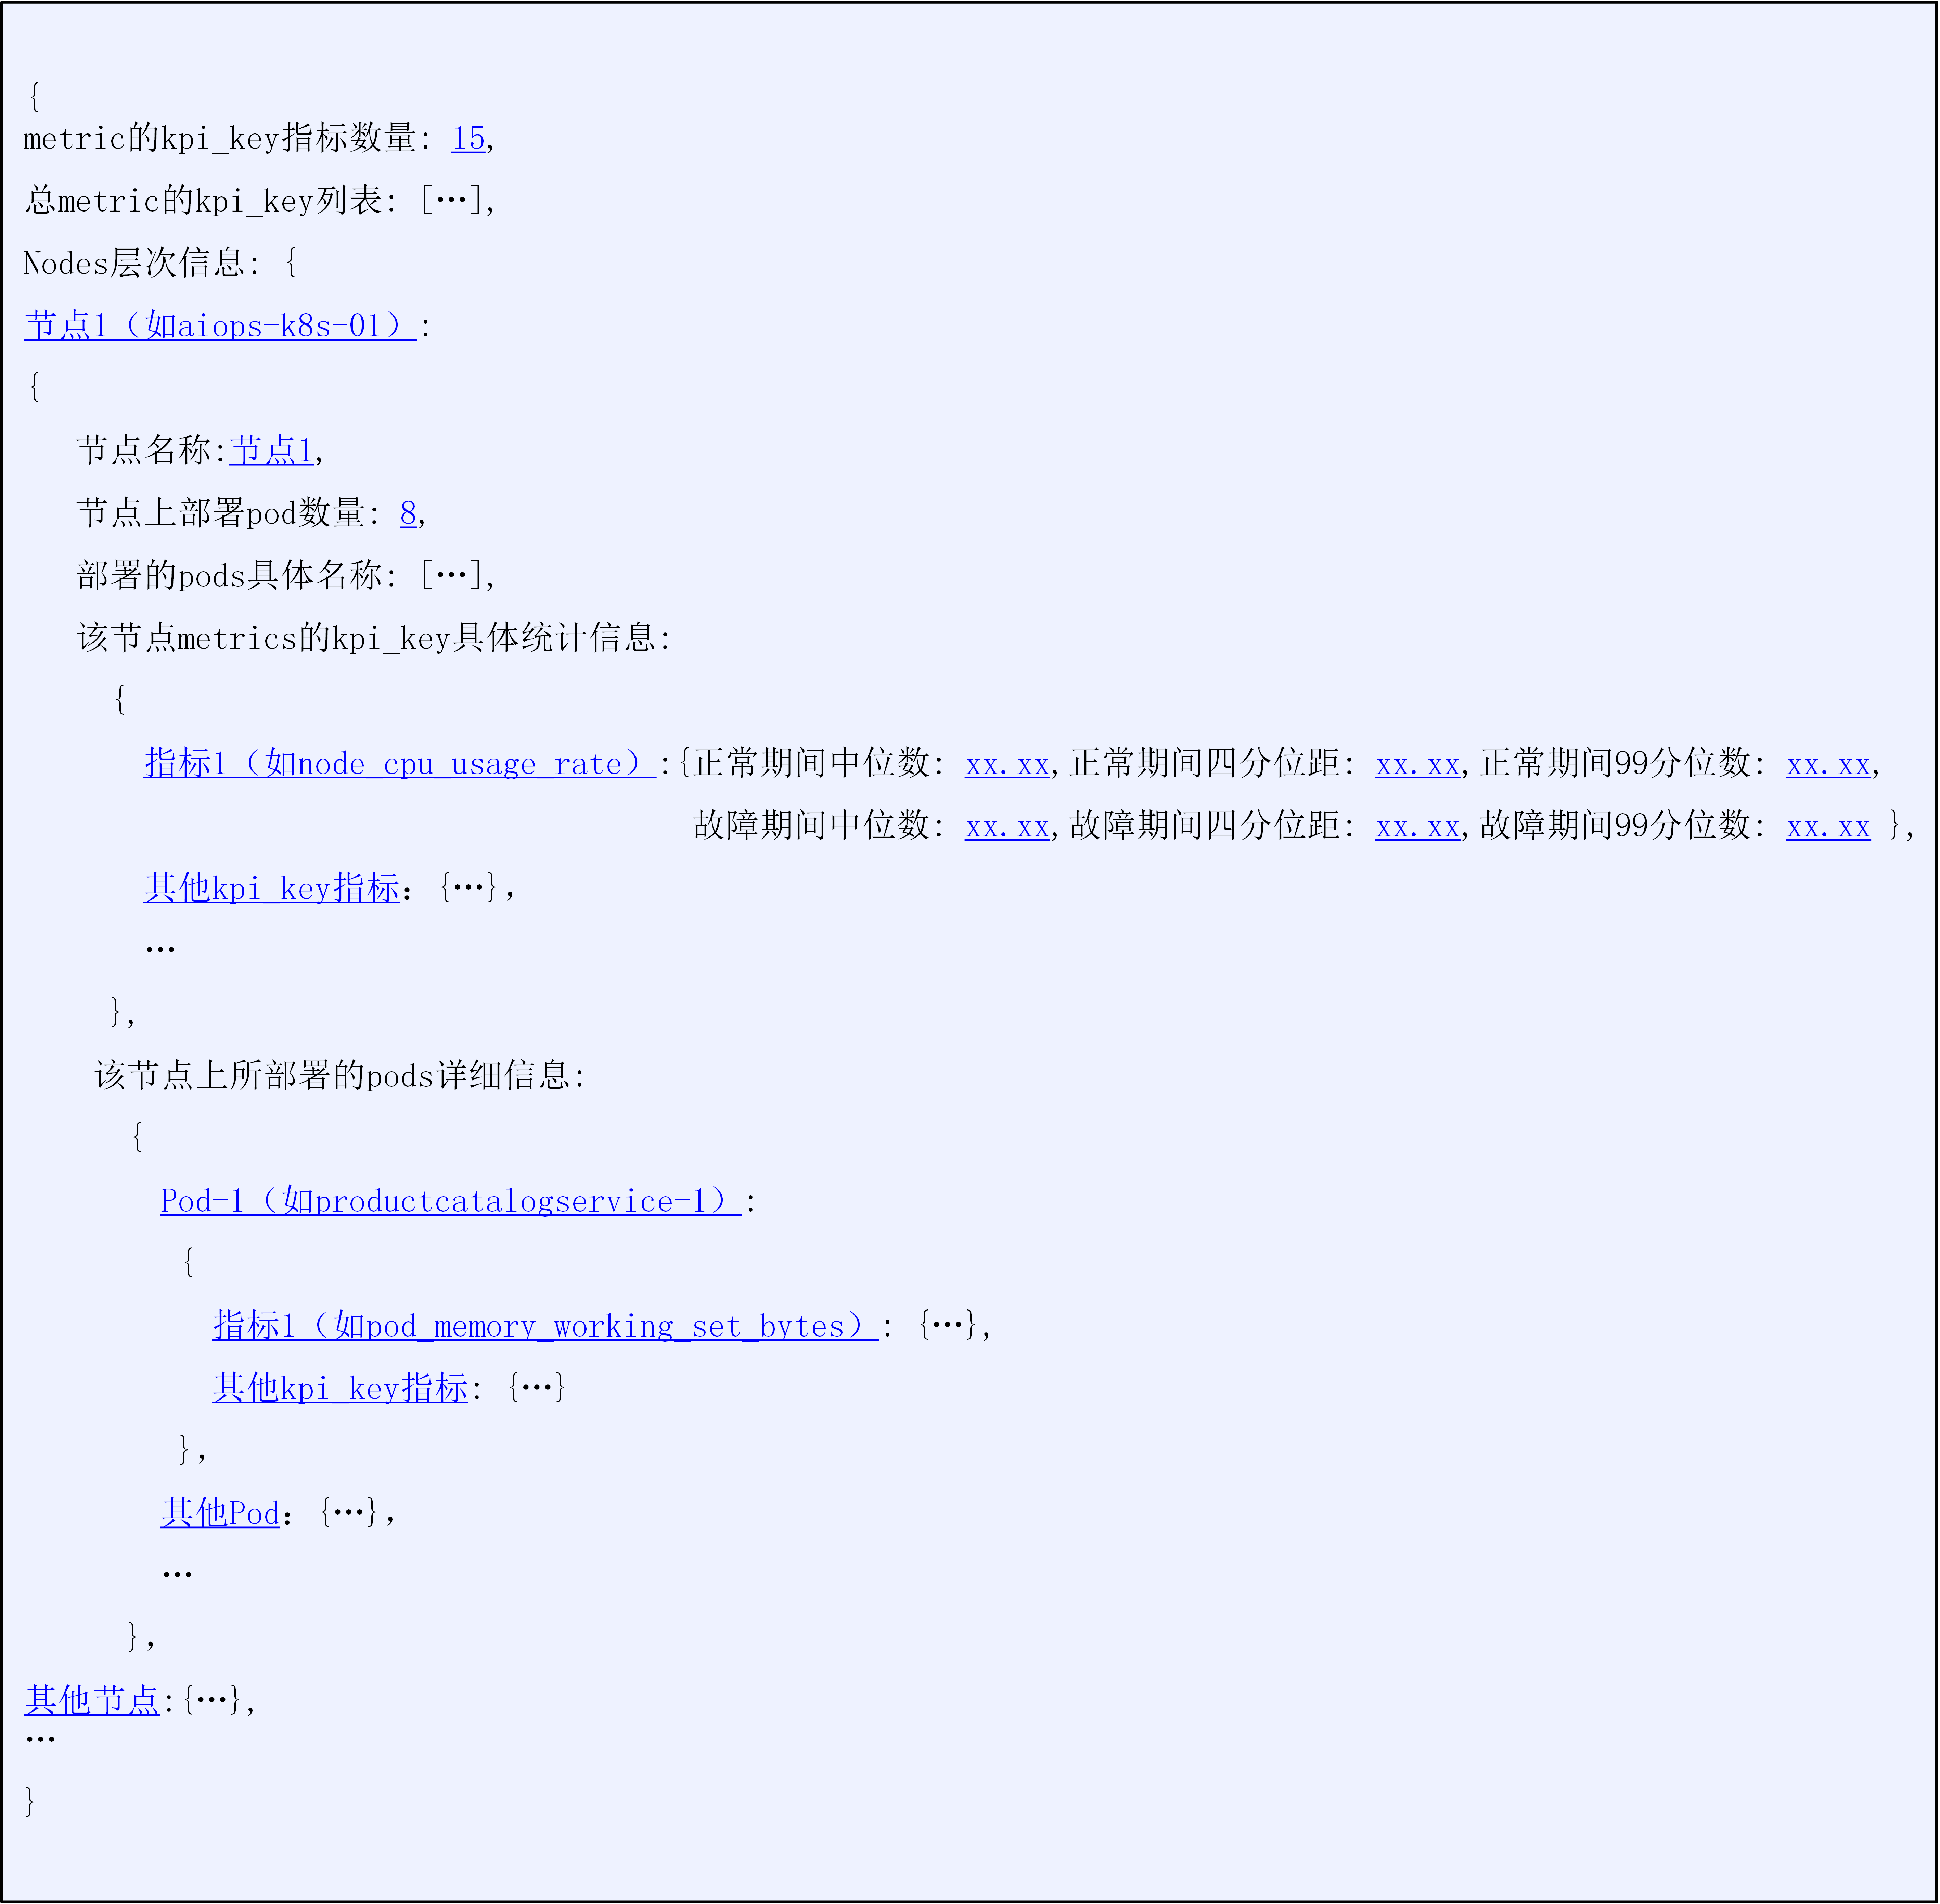
\includegraphics[width=0.95\textwidth]{pics/fig15.png}
    \caption{不同 nodes 与在其上部署的 pods 的 kpi\_key 指标统计数据对比示例}
    \label{fig15}
\end{figure*}

\begin{figure*}[htbp]
    \centering
    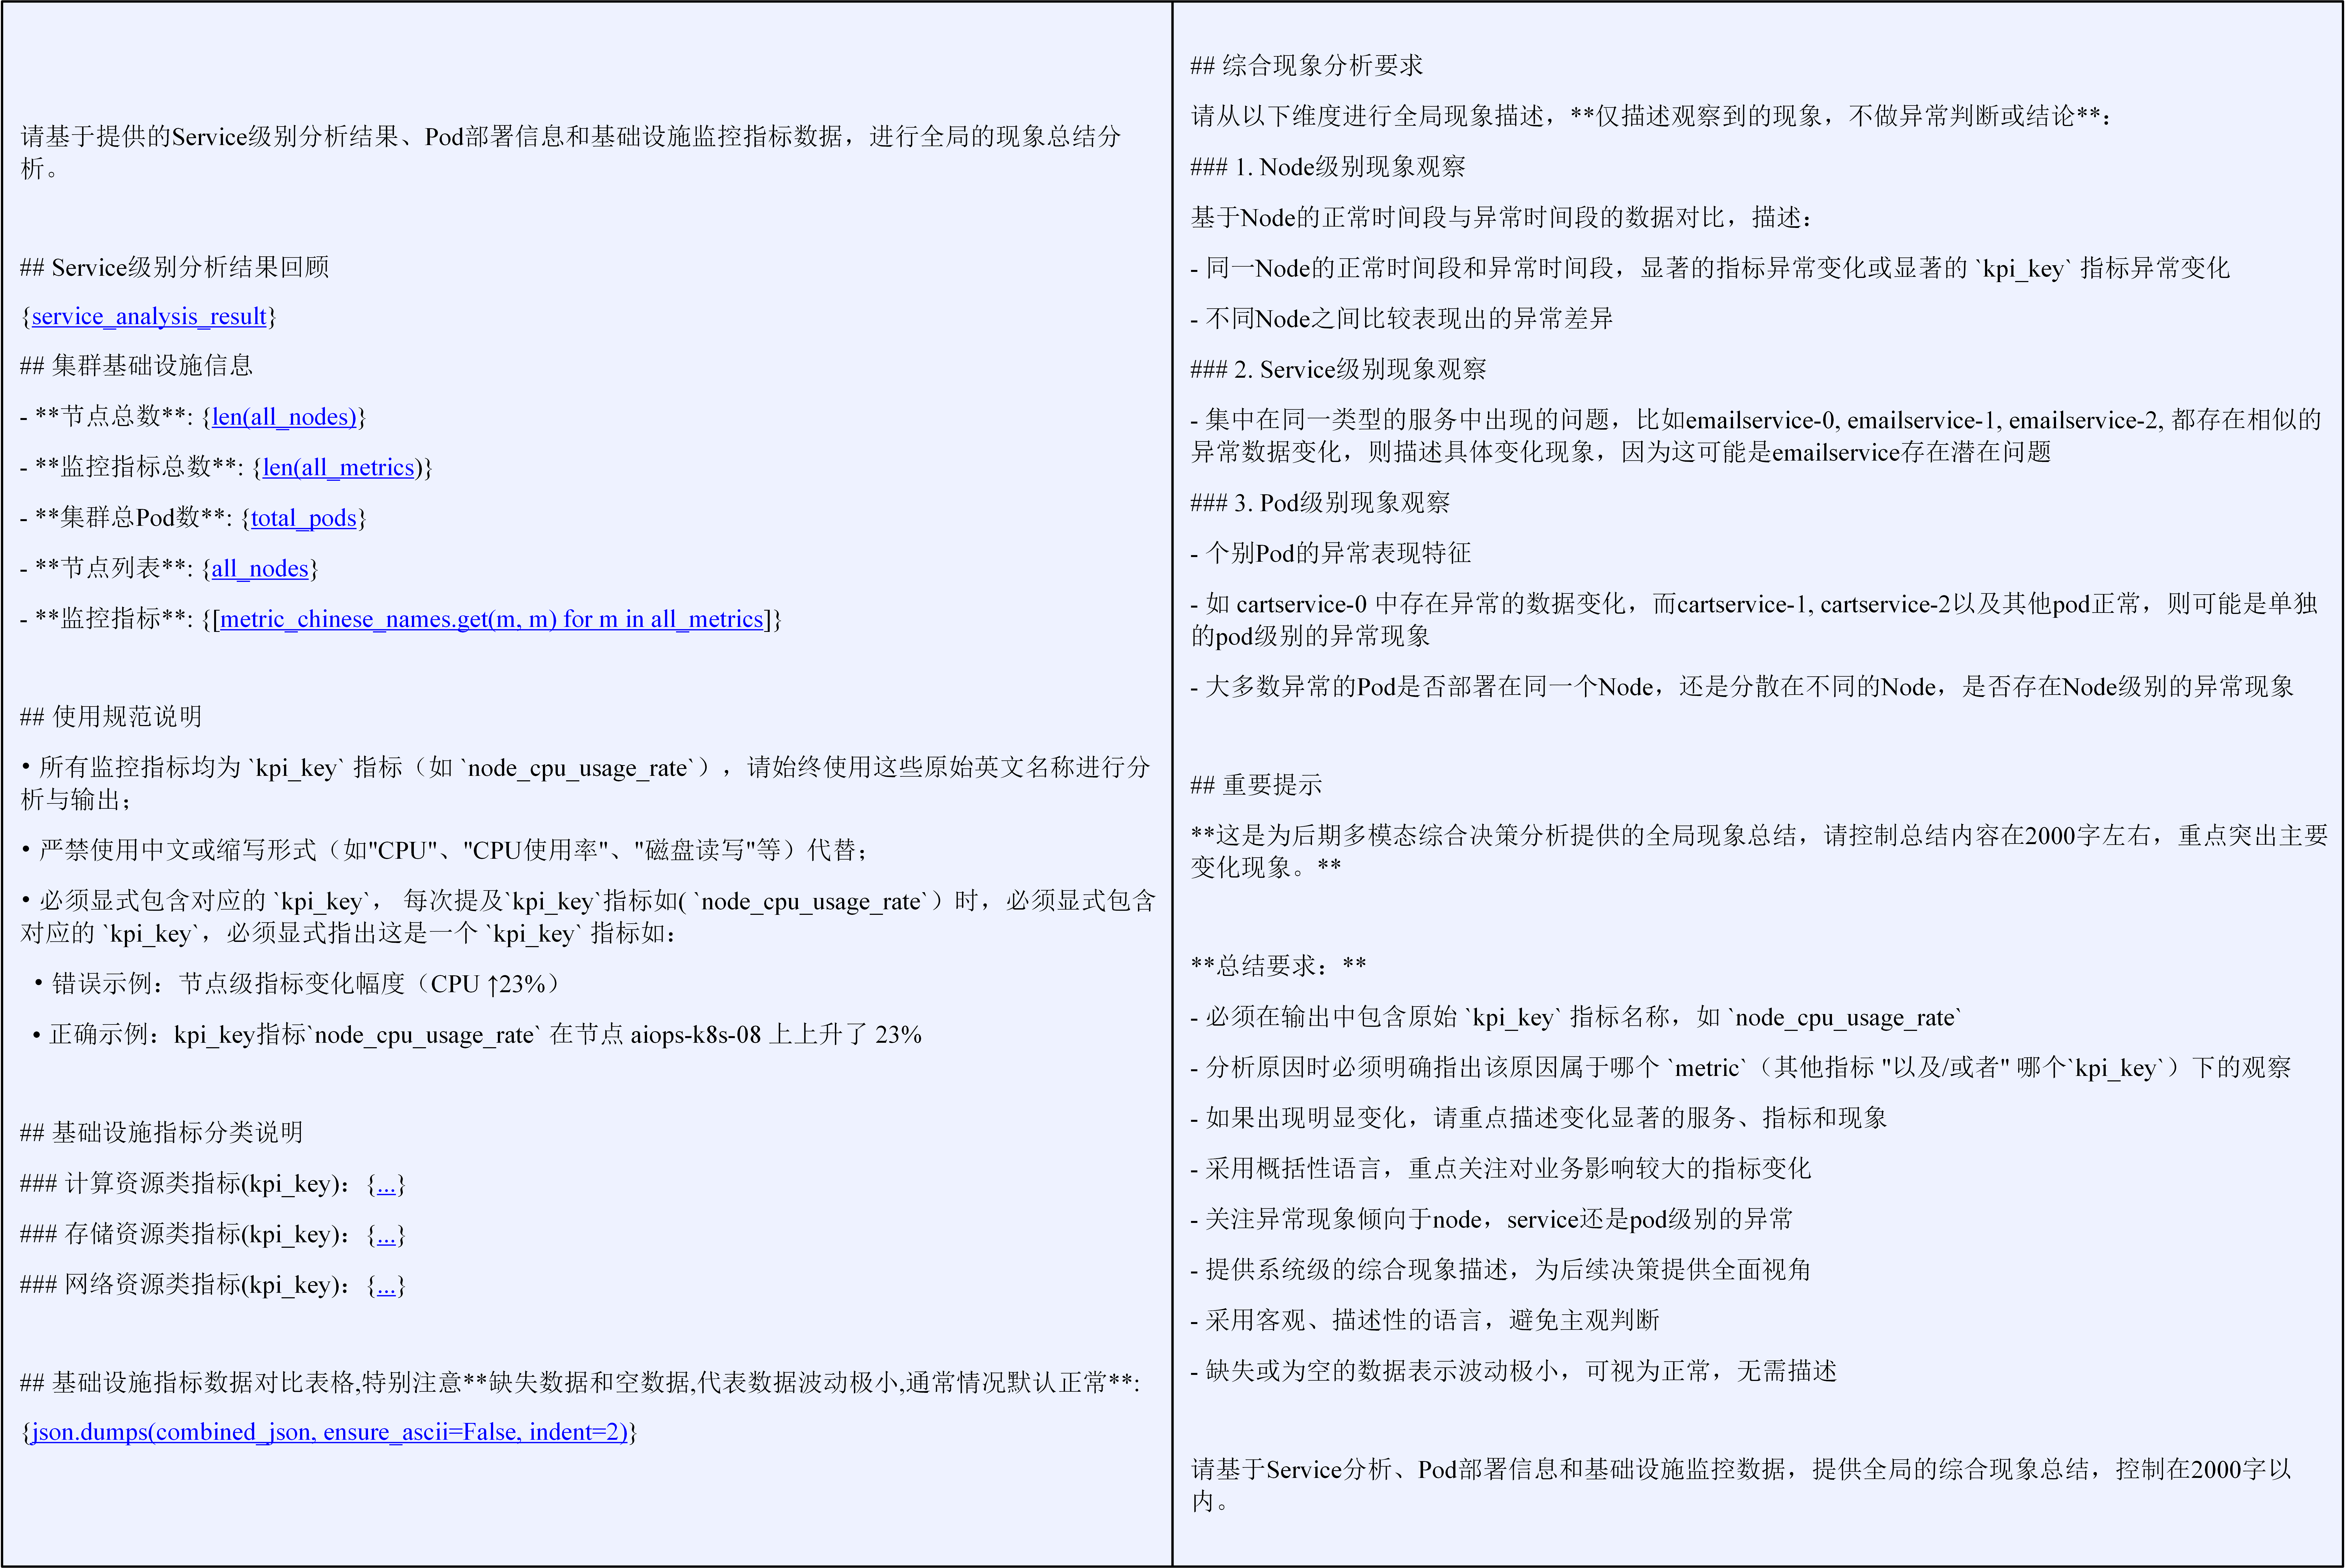
\includegraphics[width=0.95\textwidth]{pics/fig16.png}
    \caption{第二次综合现象总结 prompt}
    \label{fig16}
\end{figure*}

\paragraph{结构化现象输出与特征提取}

经过双层级大模型分析处理,metric故障总结模块输出包含以下内容的现象描述:

\textbf{应用性能异常现象:}通过service-pod的层次化信息,识别出现显著性能变化的微服务组件和数据库组件。包括request(请求数量)、response(响应数量)、rrt(平均响应时间)等请求处理指标的变化,error\_ratio(总体错误率)、client\_error\_ratio(客户端错误率)、server\_error\_ratio(服务端错误率)、timeout(超时次数)等异常指标的波动,以及TiDB组件failed\_query\_ops(失败查询数)、duration\_99th(99分位请求延迟)、connection\_count(连接数)等数据库性能指标的变化。能够同时体现服务级别的整体趋势和Pod级别的个体差异。

\textbf{基础设施机器性能异常现象:}描述容器和节点层面的资源状态变化,包括node\_cpu\_usage\_rate(节点CPU使用率)、pod\_cpu\_usage(Pod CPU使用率)等计算资源指标,node\_memory\_usage\_rate(节点内存使用率)、pod\_memory\_working\_set\_bytes(Pod工作集内存使用量)等内存资源指标,node\_disk\_read\_bytes\_total(磁盘读取字节数)、node\_disk\_written\_bytes\_total(磁盘写入字节数)、pod\_fs\_reads\_bytes(Pod文件系统读取字节数)等存储资源指标,node\_network\_receive\_bytes\_total(网络接收字节数)、node\_network\_transmit\_bytes\_total(网络发送字节数)、pod\_network\_receive\_bytes(Pod网络接收字节数)等网络资源指标的变化模式,以及异常分布在不同节点和容器间的空间特征。

\textbf{跨层级关联现象模式:}通过Pod部署拓扑和现象关联分析,识别服务异常与基础设施异常之间的关联模式,判断异常现象的分布特征和传播路径,为后续结合log和trace数据的多模态故障根因分析提供重要的现象线索。

通过上述系统化的处理流程,metric故障总结模块实现了从海量多维监控数据到精炼现象描述的转换。该模块充分发挥了大语言模型的语义理解和推理能力,专注于现象总结而非故障判断,不仅显著提升了异常现象识别的准确性和完整性,还为后续结合多模态数据的故障根因分析提供了高质量的语义化metric数据基础。

metric故障总结模块输出样例具体如\ref{fig17}所示。

\begin{figure*}[htbp]
    \centering
    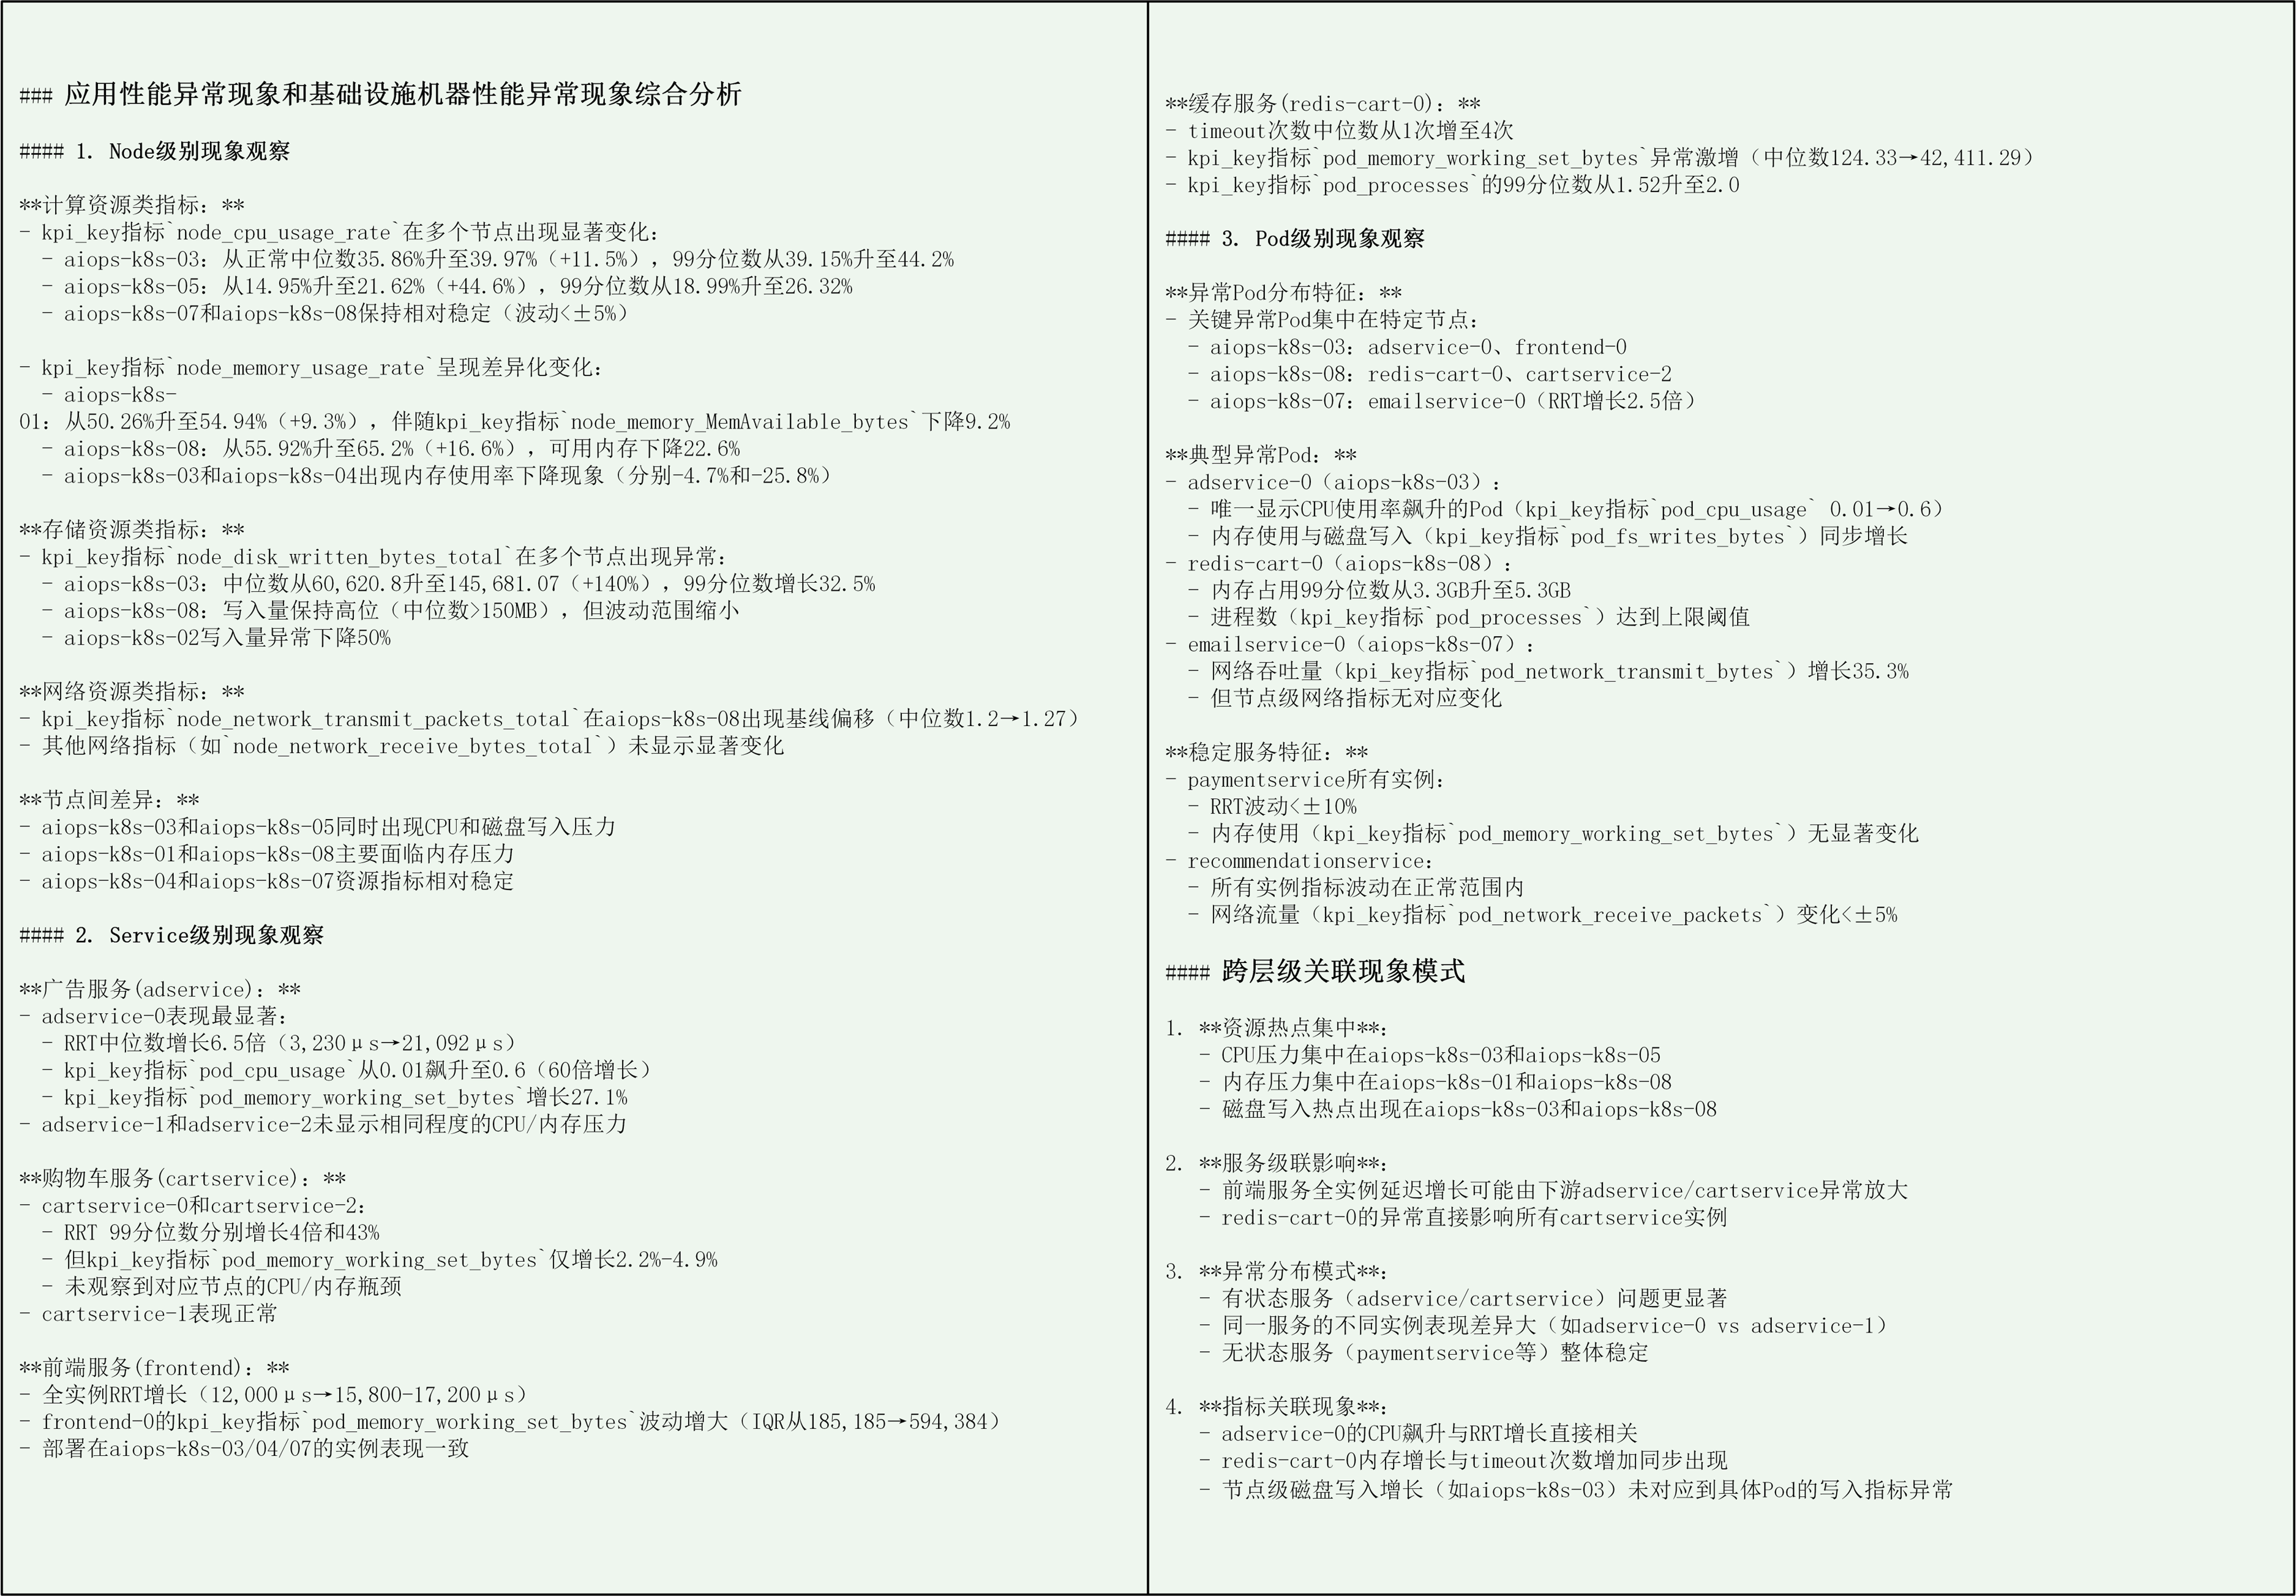
\includegraphics[width=0.95\textwidth]{pics/fig17.png}
    \caption{metric 故障总结模块输出示例}
    \label{fig17}
\end{figure*}

\subsection{多模态根因分析}

多模态根因分析模块是微服务系统故障根因定位的核心决策组件,采用基于大语言模型的综合推理策略,将经过预处理的log故障数据、trace异常模式和metric现象总结进行综合分析,实现从多维度异常信息到精准根因定位的自动化推理。该模块充分利用大语言模型的跨模态理解能力和逻辑推理能力,为复杂微服务故障提供最终的组件定位和原因解释。

\subsubsection{输入数据整合}

系统首先对三种模态的处理结果进行整合。Log故障抽取模块基于drain日志解析算法结合多重筛选机制,将海量原始日志压缩为高质量故障特征;Trace故障检测模块输出两部分异常信息,duration异常检测结果包含前20个最频繁的IsolationForest识别异常,涵盖调用关系、性能对比和异常统计,status异常检测结果包含前20个最频繁的状态码异常,涵盖错误类型和具体描述;Metric故障总结模块输出经过双层级大模型分析的现象描述总结,包含约2000字的详细异常现象描述,涵盖node、service、pod多层级的监控异常模式。

\subsubsection{多模态 prompt 生成}

基于整合后的多模态数据,系统构建专门的跨模态分析prompt模板。prompt设计遵循结构化原则,明确标识各模态数据的来源、类型和分析重点,为大语言模型提供清晰的数据理解指导。同时在prompt中明确输出要求和格式规范,确保大模型能够基于多模态证据链进行系统化的根因推理,prompt设计如\ref{fig18}所示。

\begin{figure*}[htbp]
    \centering
    \includegraphics[width=0.95\textwidth]{pics/fig18.png}
    \caption{多模态分析 prompt}
    \label{fig18}
\end{figure*}

\subsubsection{结构化输出格式设计}

系统主要通过给出输出样例提示词引导标准化的输出格式,确保根因分析结果的一致性和可解释性。输出结果包含三个核心字段:故障组件(component)、故障原因(reason)和推理过程(reasoning\_trace)。故障组件字段明确标识出问题的微服务组件名称,故障原因字段提供简介明确的根因描述,推理过程字段详细记录模型的分析逻辑和证据链条,为结果验证和后续优化提供依据。

\subsubsection{结果提取与验证机制}

由于大模型输出结果可能具有不稳定性(比如最后缺少返括号,包含多余的解释等),系统采用正则表达式和结构化解析方法从大语言模型的自然语言输出中提取标准化结果。通过JSON格式验证确保输出结果的格式正确,通过内容完整性检查确保关键字段的有效性。对于解析失败或格式不符的结果,系统提供重试和异常处理流程,最大程度保障输出质量。

通过上述多模态根因分析流程,系统实现了从异构监控数据到故障定位的端到端自动化处理。该模块充分发挥了大语言模型在跨模态理解和逻辑推理方面的优势,为复杂微服务系统的故障根因定位提供了高效、准确、可解释的解决方案。

\section{结果分析}

\subsection{Good case 与 bad case 对比}

\begin{figure*}[htbp]
    \centering
    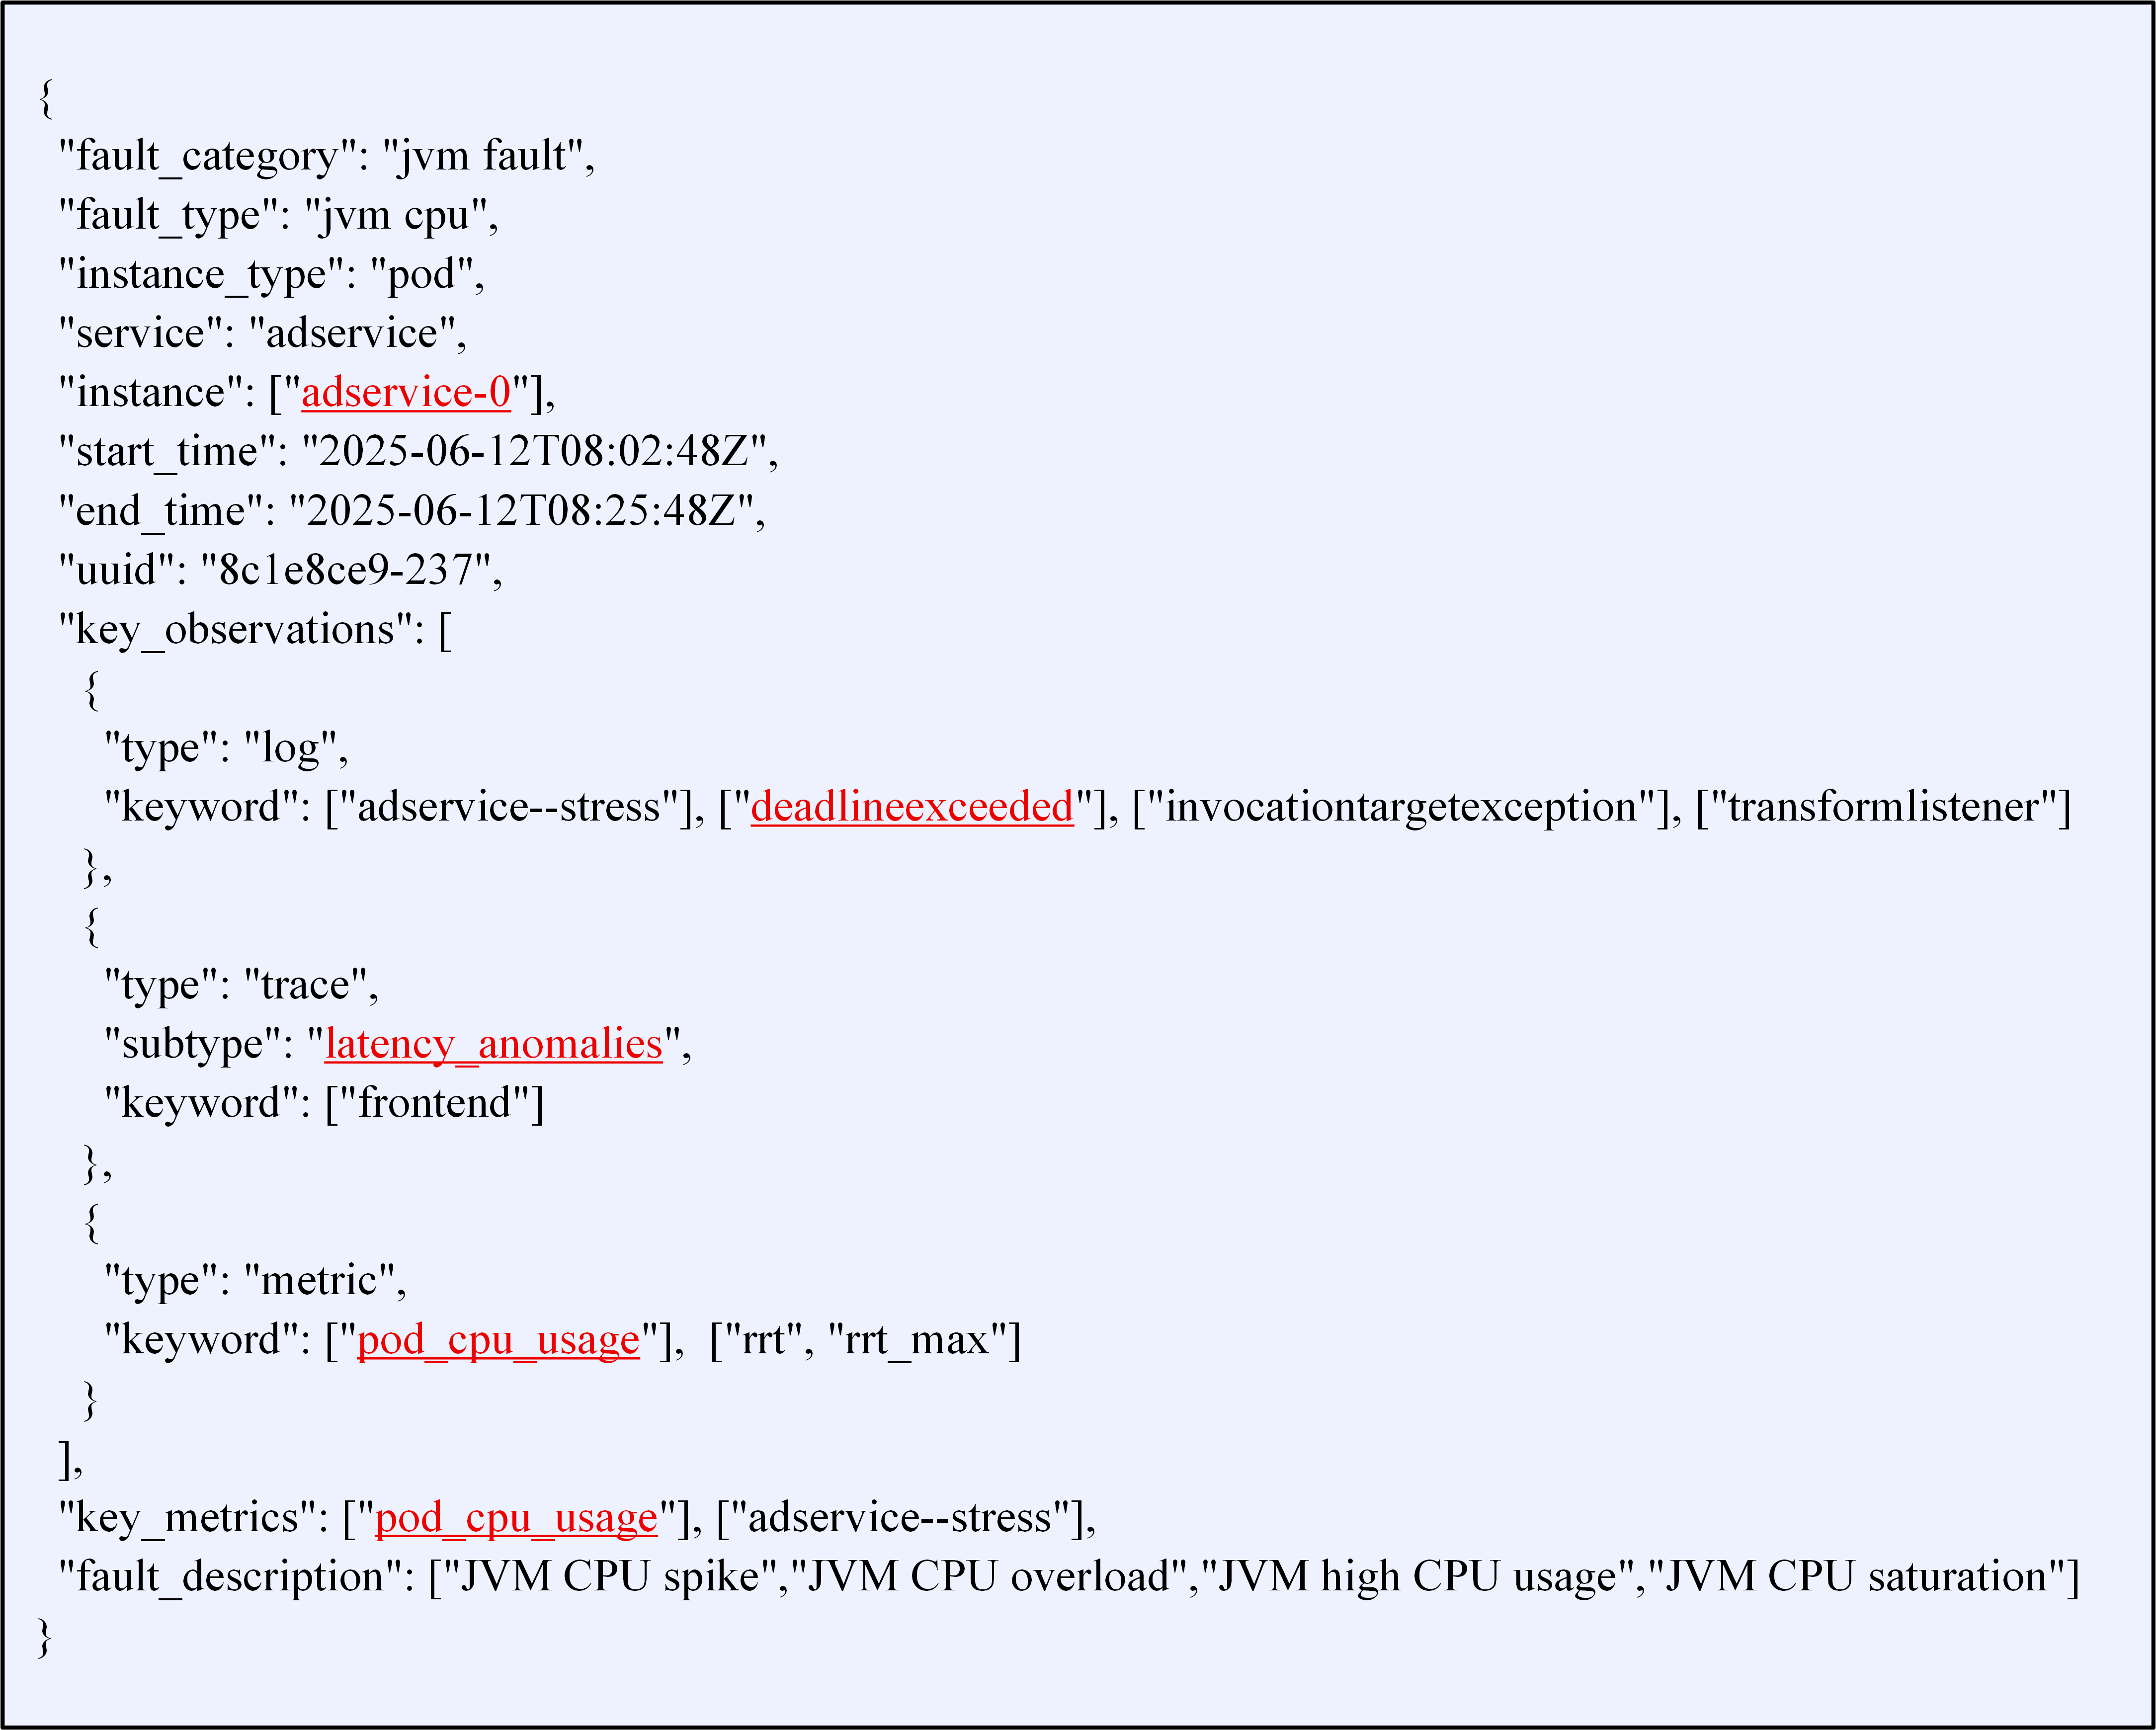
\includegraphics[width=0.95\textwidth]{pics/fig19.png}
    \caption{Good case 真实值范围}
    \label{fig19}
\end{figure*}

\begin{figure*}[htbp]
    \centering
    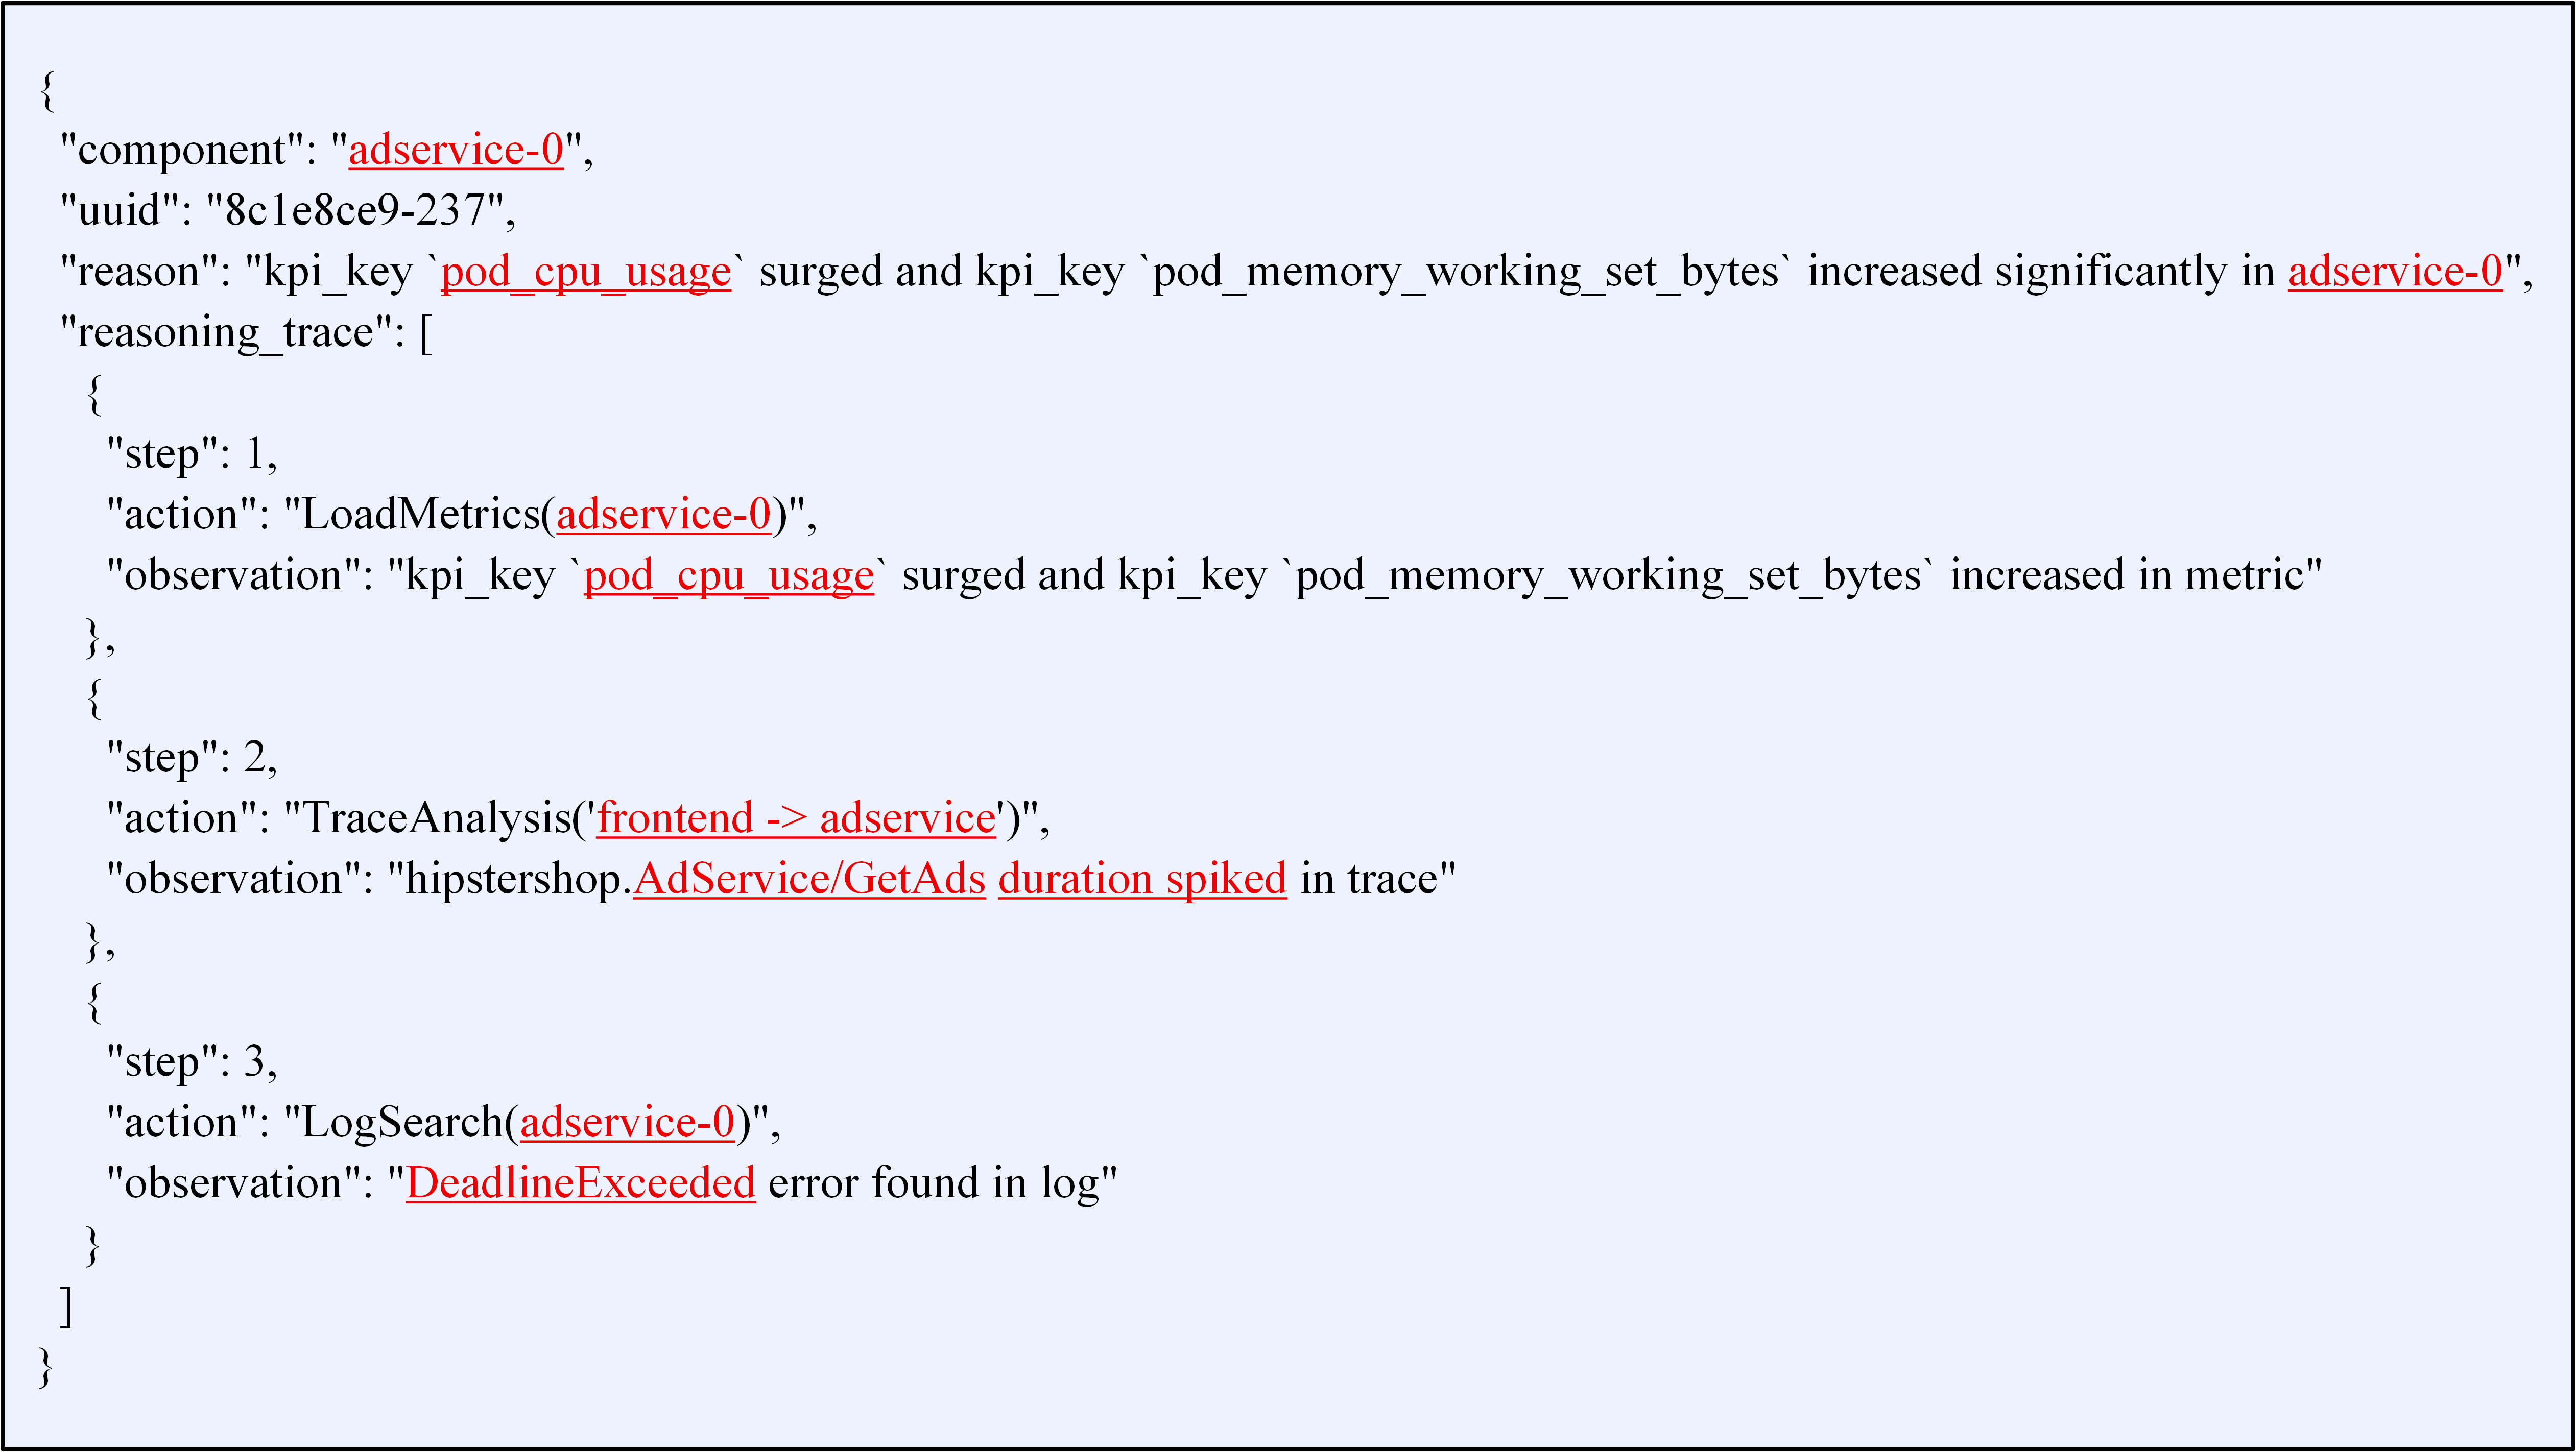
\includegraphics[width=0.95\textwidth]{pics/fig20.png}
    \caption{Good case 实际输出值}
    \label{fig20}
\end{figure*}

如\ref{fig19}和\ref{fig20}所示,所提出的多模态数据融合的智能故障根因定位系统,通过深度整合日志、链路追踪和系统指标三种监控数据能,够精准识别三种模态数据的最可能的故障组件和关键根因的推导证据,这证明了设计的多模态提取方案均有效实行。此外,方案能够作出合理的顺序推理,并能有效识别故障层次类型,判断可能异常数据指标的实际层次来源(pods,service,nodes)。最终,多模态根因分析模块能够从 log故障数据、trace异常模式和metric现象三类数据的中做出合理的故障根因判断,将大预言模型的多模态分析和逻辑推理判断能力有效结合,实现合理故障根因定位的目标。

\begin{figure*}[htbp]
    \centering
    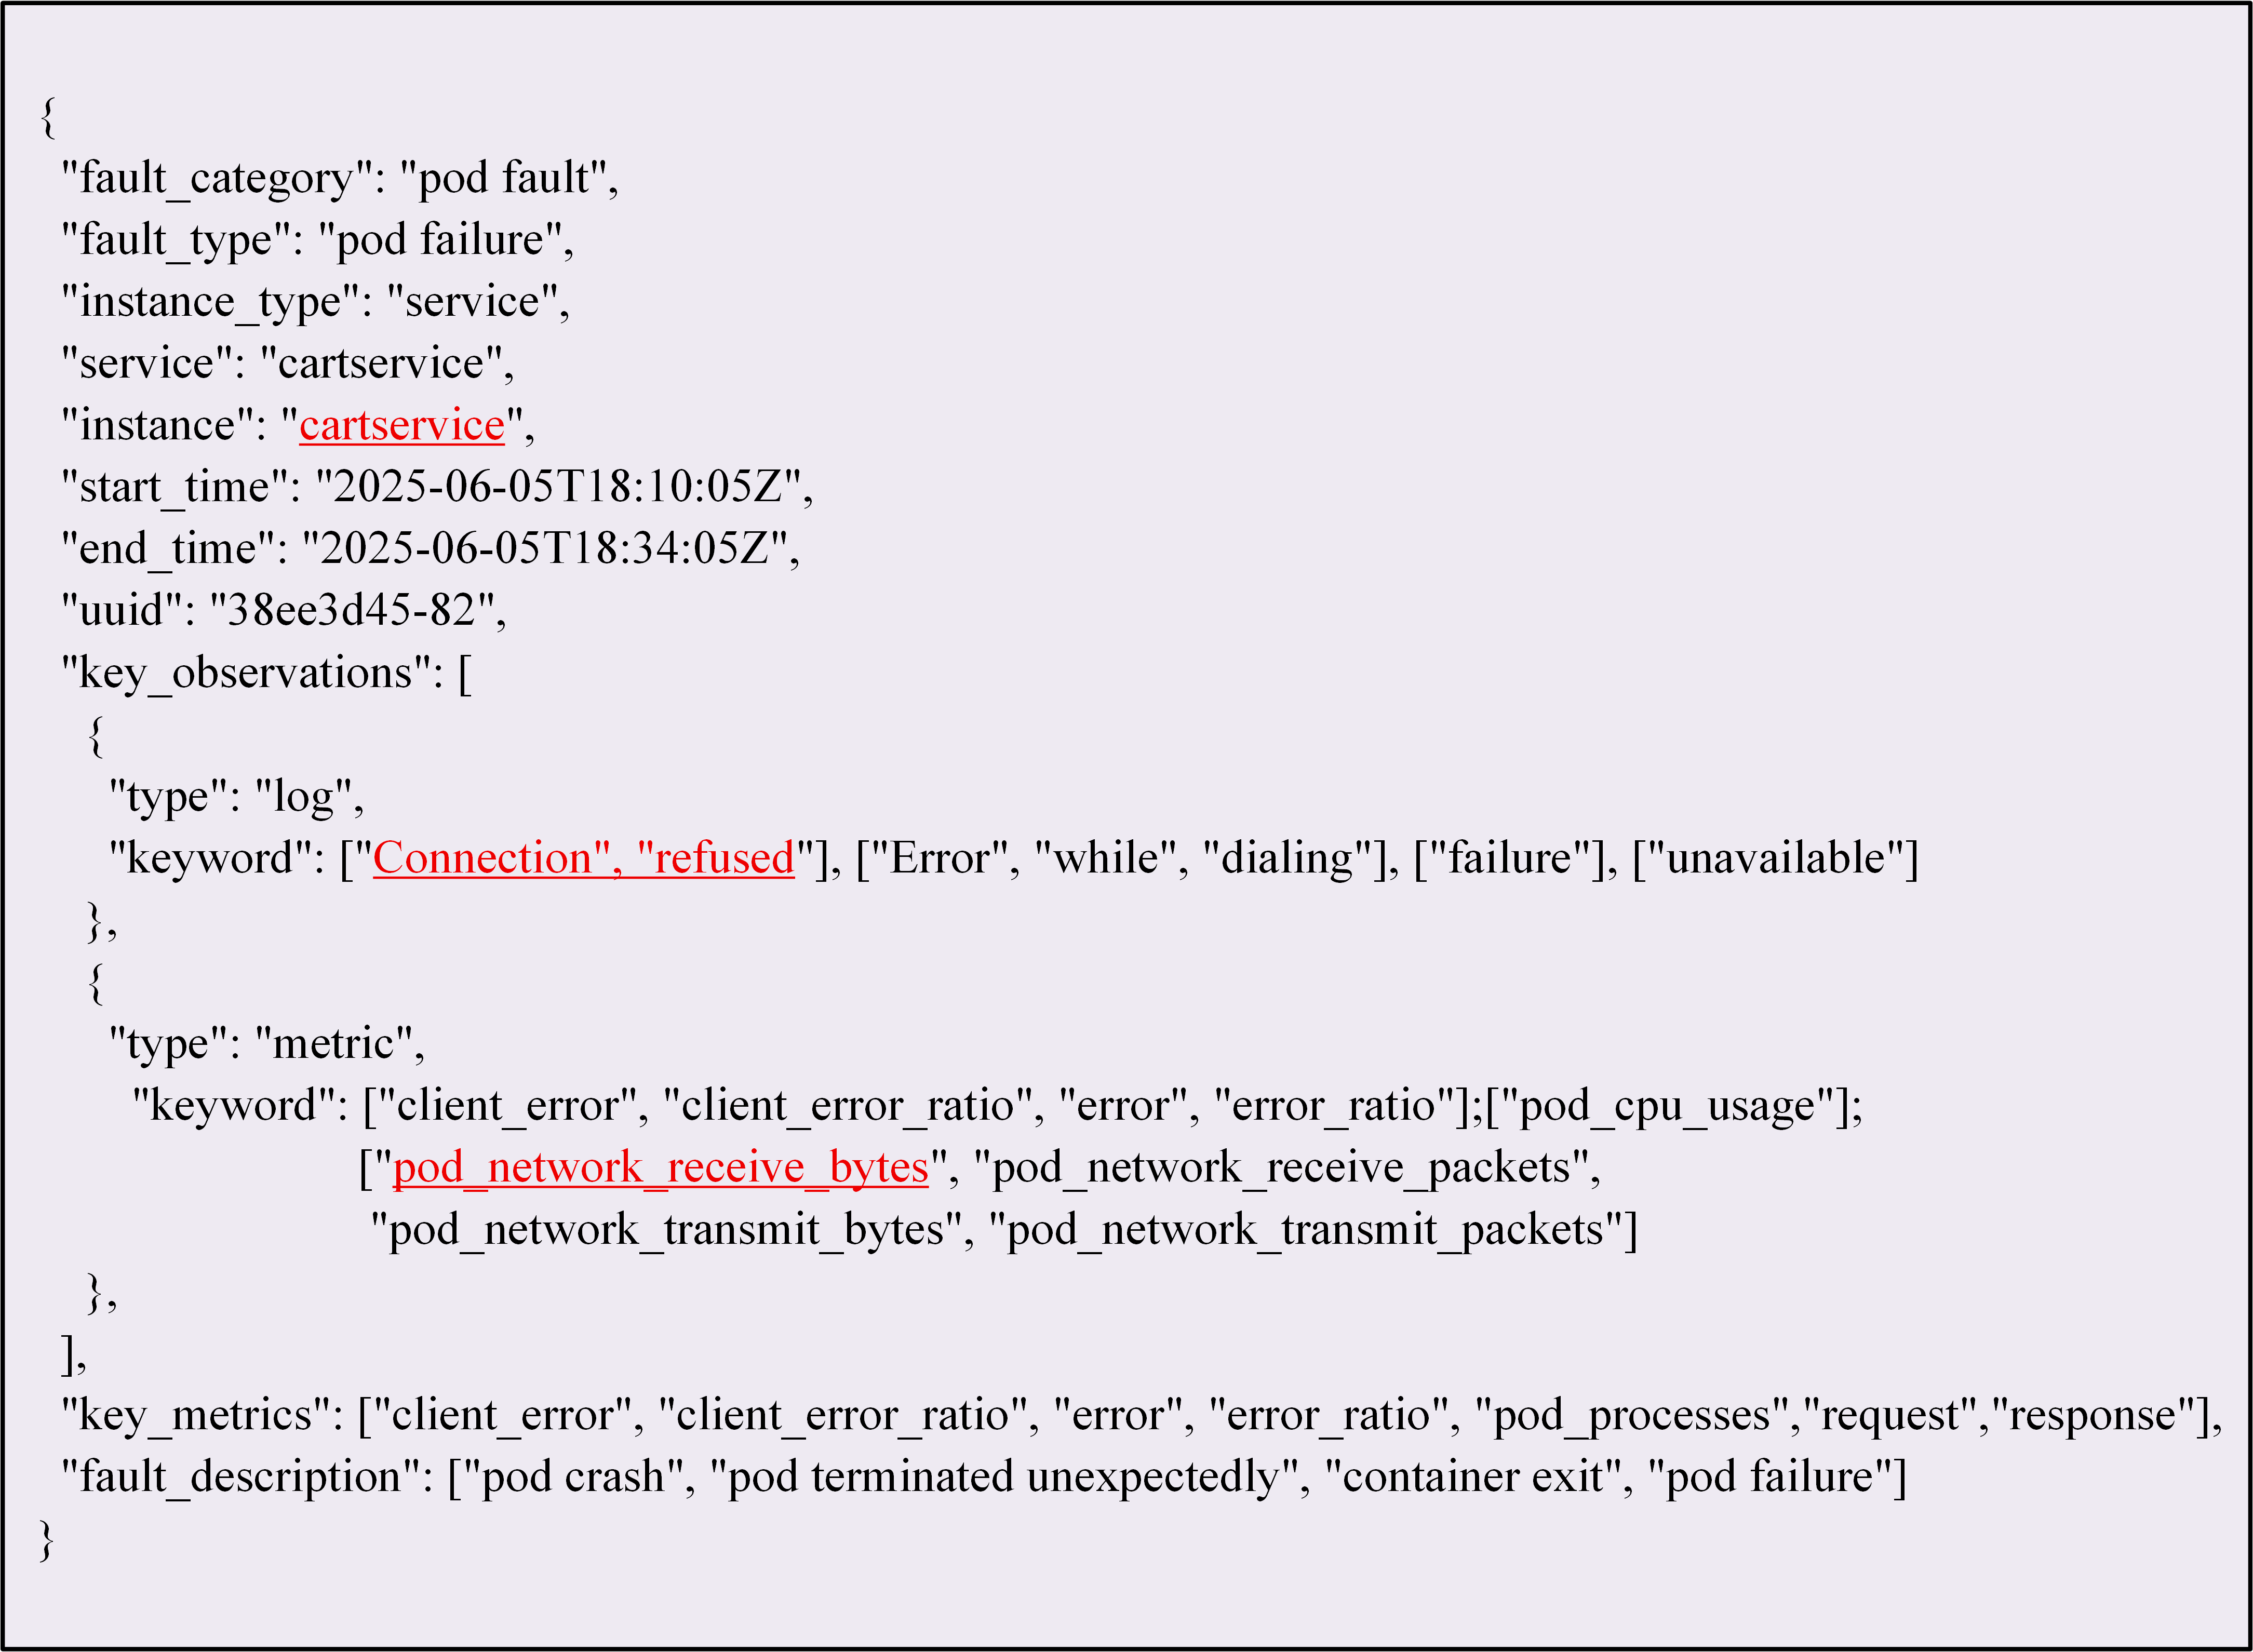
\includegraphics[width=0.95\textwidth]{pics/fig21.png}
    \caption{Bad case 真实范围值}
    \label{fig21}
\end{figure*}

\begin{figure*}[htbp]
    \centering
    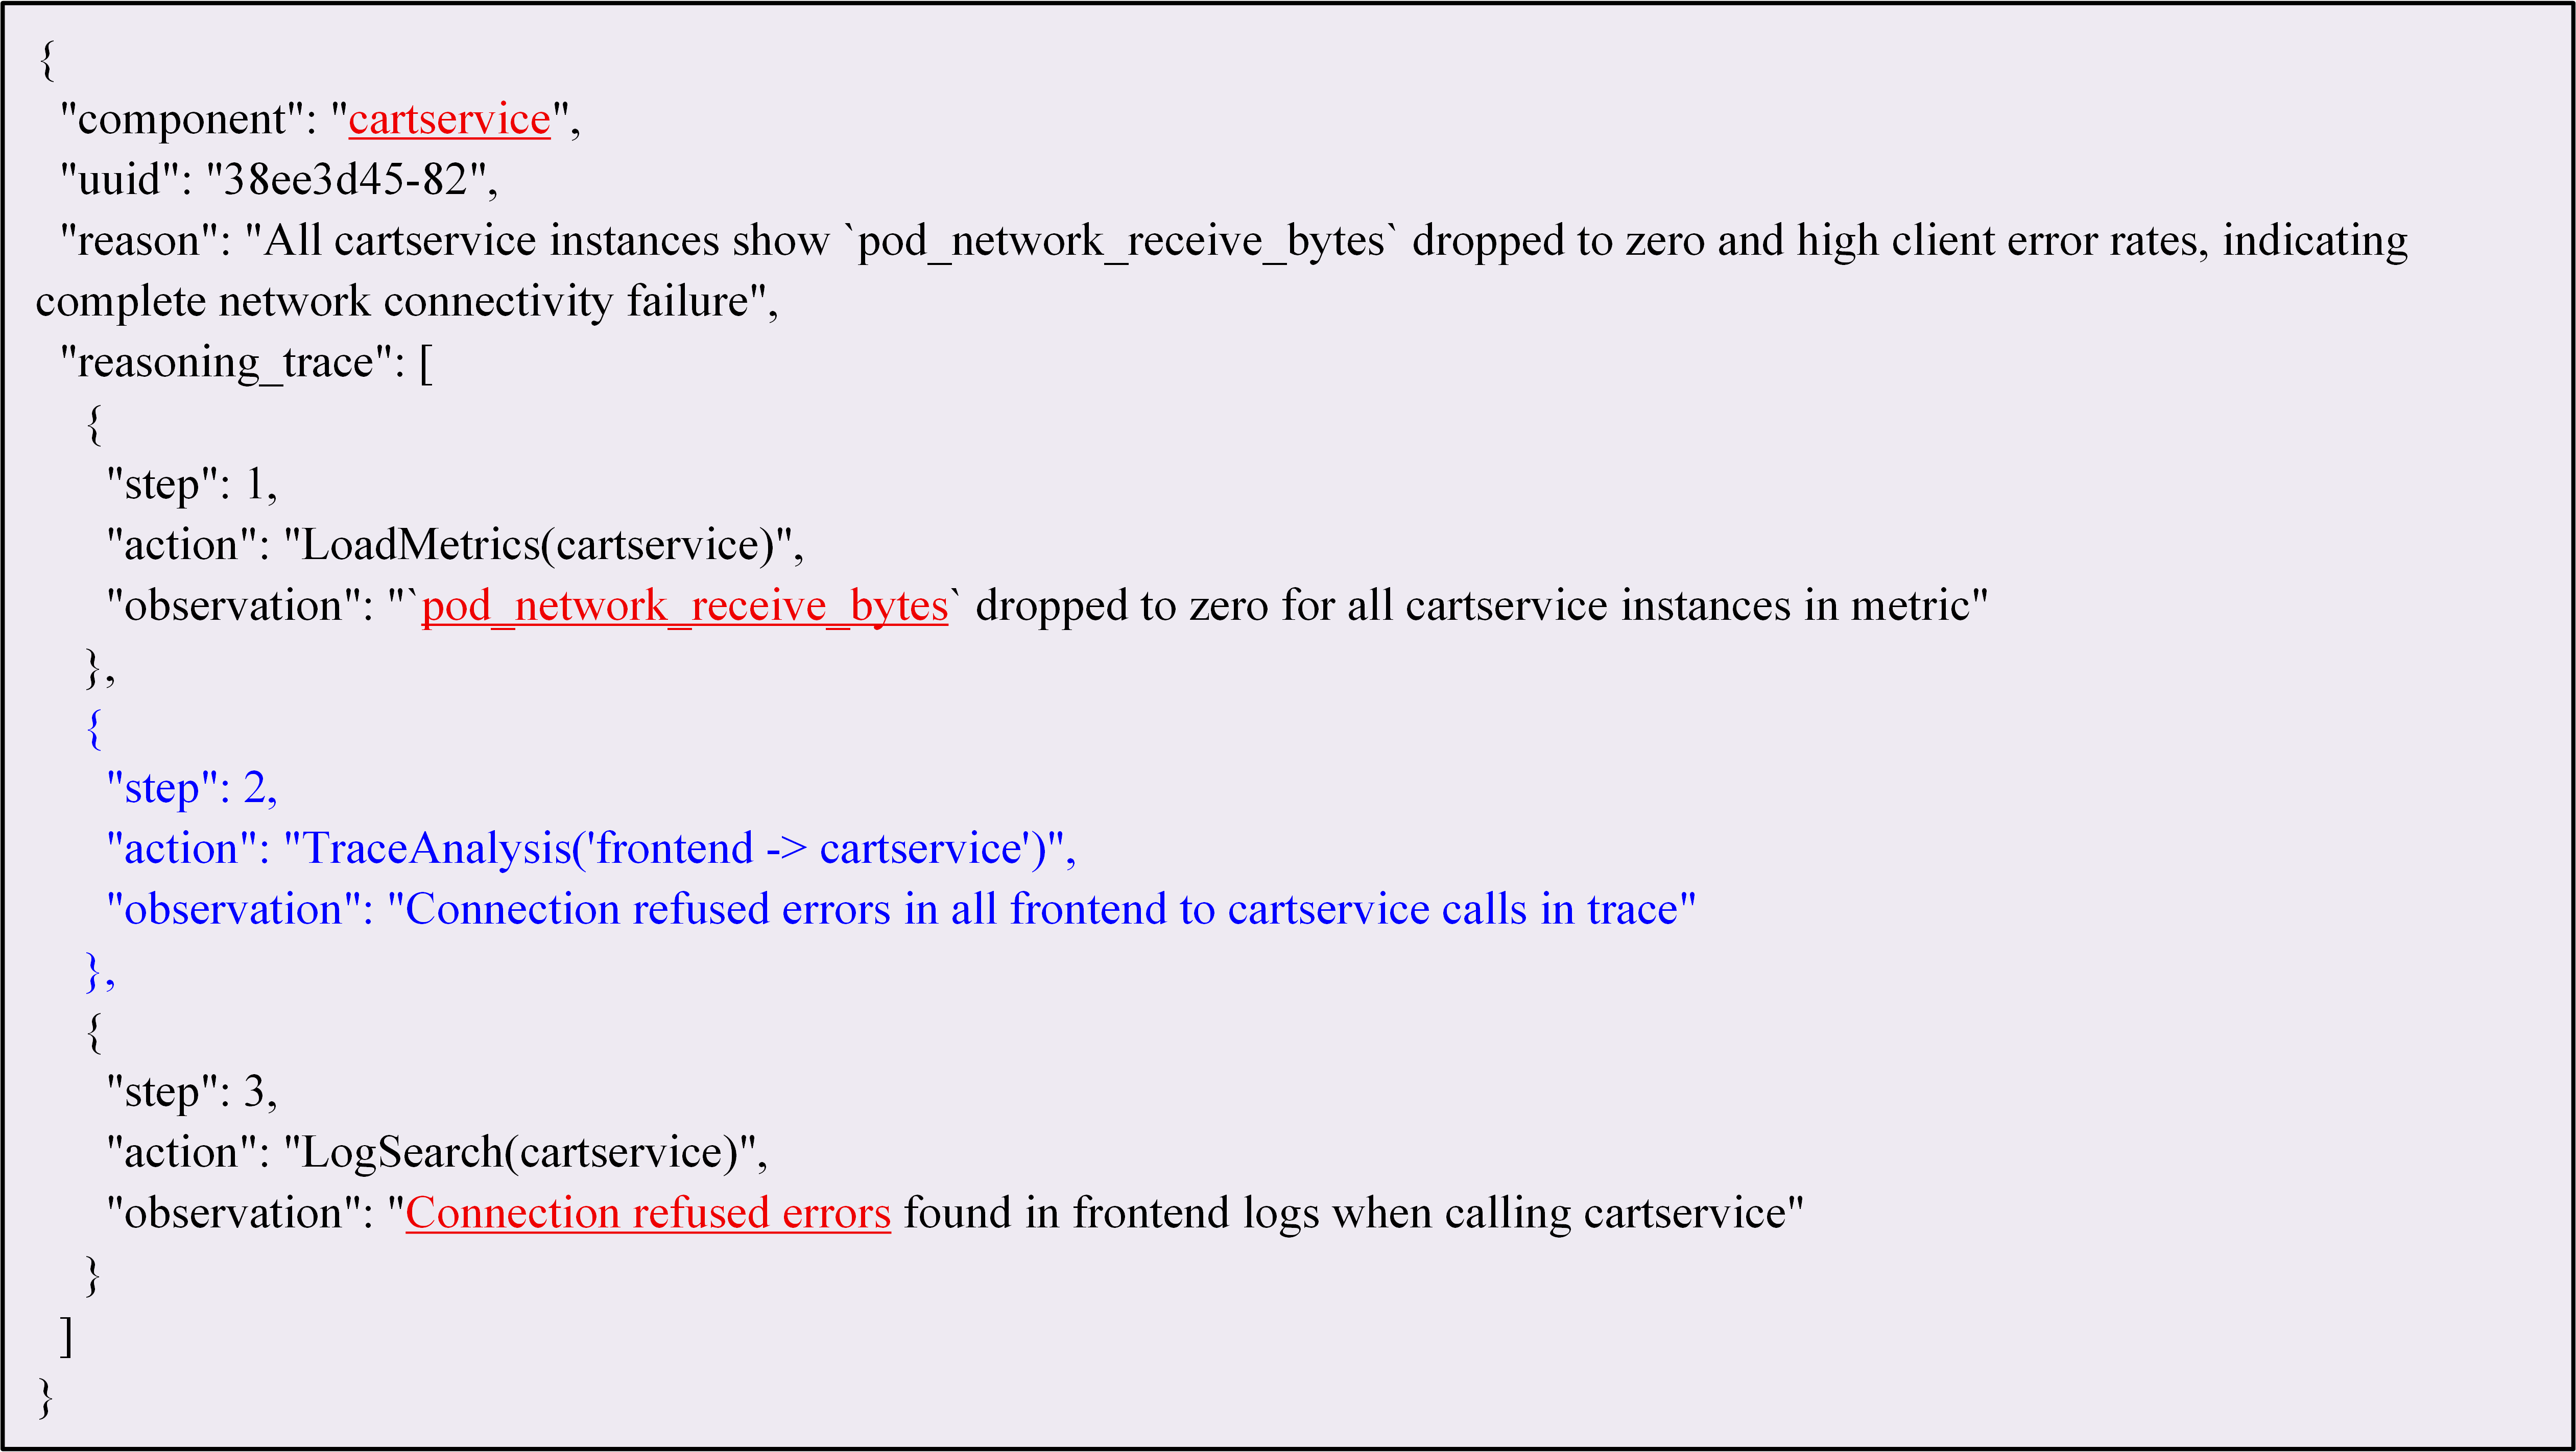
\includegraphics[width=0.95\textwidth]{pics/fig22.png}
    \caption{Bad case 实际输出值}
    \label{fig22}
\end{figure*}

此外我们还探索了典型bad case 以进一步研究方案的提升空间,如\ref{fig21}和\ref{fig22}所示,大模型在最终进行根因分析时出现了幻觉现象(图中蓝色所示),相关trace调用链实际未传入大模型进行根因分析,从而导致错误的推导链。这可能导致在最终在故障根因判断时出现偏差,影响方案稳定性。后续或采用添加检索增强生成,陪审团机制等方式进行优化。此外log相关模块能够在比赛公布答案后,通过更加广泛和具有代表性的故障数据上进一步大模型语义判断等方式生成更有效的关键词过滤模板,以此增强log筛选能力。

\subsection{消融实验分析}

\begin{table}[htbp]
\centering
\caption{各组件消融实验}
\begin{tabular}{cccc}
    \toprule
    Log & Trace & Metric & 得分 \\
    \midrule
    \textcolor{red}{\checkmark} & $\times$ & $\times$ & 23.59 \\
    \midrule
    $\times$ & \textcolor{red}{\checkmark} & $\times$ & 31.09 \\
    \midrule
    $\times$ & $\times$ & \textcolor{red}{\checkmark} & 42.78 \\
    \midrule
    \textcolor{red}{\checkmark} & \textcolor{red}{\checkmark} & $\times$ & 35.32 \\
    \midrule
    $\times$ & \textcolor{red}{\checkmark} & \textcolor{red}{\checkmark} & 48.58 \\
    \midrule
    \textcolor{red}{\checkmark} & $\times$ & \textcolor{red}{\checkmark} & 51.27 \\
    \midrule
    \textcolor{red}{\checkmark} & \textcolor{red}{\checkmark} & \textcolor{red}{\checkmark} & 50.71 \\
    \bottomrule
\end{tabular}
\label{tab:ablation}
\end{table}

为深入研究方案各组件间的协同配合机制,我们开展了系统性的消融实验,通过对比不同模态组合的性能表现,揭示了各模块的独特价值和互补关系。从表 1的实验结果可以看出,在单模态实验中,metric模块表现最为突出(42.78分),主要归因于其双层级LLM分析策略能够有效覆盖service、pod、node三个层次的全栈监控视角;trace模块表现次之(31.09分),在调用链分析和服务间依赖关系识别方面展现出较强能力;而log模块单独表现相对较弱(23.59分),主要因为日志数据的非结构化特性限制了其独立分析的准确性。双模态组合实验揭示了显著的协同效应:log+metric组合效果最佳(51.27分),这种强协同效应源于metric提供量化性能异常定位而log提供丰富的故障语义描述,两者形成了从数值异常到语义解释的完美互补;trace+metric组合次之(48.58分),两者在性能监控维度具有天然相关性;log+trace组合表现相对较弱(35.32分),缺乏metric模块的量化支撑。完整的三模态融合系统达到50.71分,虽然略低于最佳双模态组合log+metric的51.27分,但仍显著优于其他组合方式,表明log和metric的协同作用已能覆盖大部分故障模式,而trace模块在复杂调用链异常场景下仍具有独特价值。消融实验结果充分验证了本方案多模态融合架构的科学性,确认了metric模块作为系统核心分析引擎的关键地位,证明了log+metric组合的最优性能表现,为构建准确、可解释的基于大模型智能体的微服务故障根因定位解决方案提供了重要的实证支撑。

\section{总结}

本方案围绕微服务系统的故障根因定位构建了一个大模型智能体分析框架,整体由五大模块组成:数据预处理、日志故障抽取、调用链异常检测、指标现象总结与多模态根因分析。首先,数据预处理模块实现了对故障输入的结构化解析与时间戳标准化,为多源数据融合打下基础。日志模块基于Drain算法和多层级过滤机制,提取错误模板筛选有效的结构化日志特征;调用链模块结合IsolationForest模型和状态码检查,双重检测duration和status异常;指标模块通过筛选核心业务与基础设施指标,借助大语言模型进行两层次现象总结,生成可读性强的异常描述。最终,多模态根因分析模块将log、trace与metric输出融合,以精心设计的prompt驱动大语言模型进行综合推理,输出包含故障组件、原因与推理过程的结构化根因分析结果。整套系统实现了从数据处理到根因定位决策的闭环,兼顾高效性、准确性与可解释性。

% Bibliography entries for the entire Anthology, followed by custom entries
%\bibliography{anthology,custom}
% Custom bibliography entries only
\bibliography{custom}

\end{document}
